% Autor: Alex Oster, Jonathan Sigrist, Luca Wiggering
% Datum: 2018-01
% basiert auf der Vorlage für Versuchsprotokolle von Simon May

%\includeonly{
%	tex/04_Titelseite,
%	tex/05_Gliederung,
%	tex/14_Kurzfassung,
%	tex/15_Theorie,
%	tex/16_Methoden,
%	tex/17_Ergebnisse,
%	tex/19_Zusammenfassung,
%	tex/20_Anhang,
%	tex/21_Literatur
%}

\documentclass[
	a4paper,                % Papierformat (DIN A4)
	titlepage=firstiscover, % Separate Titelseite
	captions=tableheading,  % \caption bei Tabellen immer als Überschrift setzen
	toc=bibliography,       % Literaturverzeichnis im Inhaltsverzeichnis aufführen
	toc=listof,             % Abbildungsverzeichnis etc. im Inhaltsverzeichnis aufführen
	oneside,                % Einseitig
	%twoside,               % Zweiseitig
	%twocolumn,             % Zweispaltig
	automark,               % Abschnittstitel automatisch in Kopfzeile einfügen
	12pt,                   % Schriftgröße (beliebige Größen mit „fontsize=Xpt“)
	english,		% Sprache für z.B. Babel; ausgewählt: ngerman (letztgenannt)
	%draft=true             % Entwurf-Modus; markiert zu lange und zu kurze Zeilen
]{scrartcl}

% Autor: Simon May
% Datum: 2017-10-04

% --- Pakete einbinden
% --- Pakete erweitern LaTeX um zusätzliche Funktionen.
%     Dies ist ein Satz nützlicher Pakete.

% Silbentrennung etc.; Sprache wird durch Option bei \documentclass festgelegt
\usepackage{babel}
\usepackage{iftex}
\ifLuaTeX
	% Schriftart (Latin Modern)
	\usepackage{fontspec}
	\fontspec{Latin Modern Roman}
\else
	% Verwendung der Zeichentabelle T1 (für Sonderzeichen etc.)
	\usepackage[T1]{fontenc}
	% Legt die Eingabe-Zeichenkodierung fest, z.B. UTF-8
	\usepackage[utf8]{inputenc}
	% Schriftart (Latin Modern)
	\usepackage{lmodern}
	% Zusätzliche Sonderzeichen
	\usepackage{textcomp}
\fi

\usepackage{upgreek}
% Nutzen von +, -, *, / in \setlength u.ä. (z.B. \setlength{\a + 3cm})
\usepackage{calc}
% Wird benötigt, um \ifthenelse zu benutzen
\usepackage{xifthen}
% Optionen für eigene definierte Befehle
\usepackage{xparse}

% Verbessertes Aussehen des Schriftbilds durch kleine Anpassungen
\usepackage{microtype}
% Automatische Formatierung von Daten
\usepackage[useregional]{datetime2}
% Wird für Kopf- und Fußzeile benötigt
\usepackage{scrlayer-scrpage}
% Einfaches Wechseln zwischen unterschiedlichen Zeilenabständen
\usepackage{setspace}
% Optionen für Listen (enumerate, itemize, …)
\usepackage{enumitem}
% Automatische Anführungszeichen
\usepackage{csquotes}
% Zusätzliche Optionen für Tabellen (tabular)
\usepackage{array}

% Mathepaket (intlimits: Grenzen über/unter Integralzeichen)
\usepackage[intlimits]{amsmath}
% Mathe-Symbole, \mathbb etc.
\usepackage{amssymb}
% Weitere Mathebefehle
\usepackage{mathtools}
% „Schöne“ Brüche im Fließtext
\usepackage{xfrac}
% Ermöglicht die Nutzung von \SI{Zahl}{Einheit} u.a.
\usepackage{siunitx}
% Ermöglicht Nutzung von \pdv als Ableitungen
\usepackage{physics}
% Definition von Unicode-Symbolen; Nach [utf8]inputenc laden!
\usepackage{newunicodechar}
% Unicode-Formeln mit pdfLaTeX
% Autor: Simon May
% Datum: 2015-03-04

% Diese Datei ermöglicht es, Mathe-Symbole (z.B. \gamma) direkt als
% Sonderzeichen (d.h. γ) einzugeben

% silence unterdrückt Warnungen; vor hyperref laden
\usepackage{silence}
\WarningFilter[pdflatex-unicode-math]{newunicodechar}{Redefining Unicode character}
\ActivateWarningFilters[pdflatex-unicode-math]

\newunicodechar{†}{\dag}
\newunicodechar{‡}{\ddag}
\newunicodechar{…}{\ldots}
\newunicodechar{⋯}{\cdots}
\newunicodechar{⋮}{\vdots}
\newunicodechar{⋱}{\ddots}
\newunicodechar{⋰}{\iddots}
\newunicodechar{α}{\alpha}
\newunicodechar{β}{\beta}
\newunicodechar{γ}{\gamma}
\newunicodechar{δ}{\delta}
\newunicodechar{ε}{\varepsilon}
\newunicodechar{ϵ}{\epsilon}
\newunicodechar{ζ}{\zeta}
\newunicodechar{η}{\eta}
\newunicodechar{θ}{\theta}
\newunicodechar{ϑ}{\vartheta}
\newunicodechar{ι}{\iota}
\newunicodechar{κ}{\kappa}
\newunicodechar{ϰ}{\varkappa}
\newunicodechar{λ}{\lambda}
\newunicodechar{μ}{\mu}
\newunicodechar{ν}{\nu}
\newunicodechar{ξ}{\xi}
\newunicodechar{ο}{o}
\newunicodechar{π}{\pi}
\newunicodechar{ρ}{\rho}
\newunicodechar{ϱ}{\varrho}
\newunicodechar{σ}{\sigma}
\newunicodechar{τ}{\tau}
\newunicodechar{υ}{\upsilon}
\newunicodechar{φ}{\varphi}
\newunicodechar{ϕ}{\phi}
\newunicodechar{χ}{\chi}
\newunicodechar{ψ}{\psi}
\newunicodechar{ω}{\omega}
\newunicodechar{Α}{\mathrm{A}}
\newunicodechar{Β}{\mathrm{B}}
\newunicodechar{Γ}{\Gamma}
\newunicodechar{Δ}{\Delta}
\newunicodechar{Ε}{\mathrm{E}}
\newunicodechar{Ζ}{\mathrm{Z}}
\newunicodechar{Η}{\mathrm{H}}
\newunicodechar{Θ}{\Theta}
\newunicodechar{Ι}{\mathrm{I}}
\newunicodechar{Κ}{\mathrm{K}}
\newunicodechar{Λ}{\Lambda}
\newunicodechar{Μ}{\mathrm{M}}
\newunicodechar{Ν}{\mathrm{N}}
\newunicodechar{Ξ}{\Xi}
\newunicodechar{Ο}{\mathrm{O}}
\newunicodechar{Π}{\Pi}
\newunicodechar{Ρ}{\mathrm{P}}
\newunicodechar{Σ}{\Sigma}
\newunicodechar{Τ}{\mathrm{T}}
\newunicodechar{Υ}{\Upsilon}
\newunicodechar{Φ}{\Phi}
\newunicodechar{Χ}{\Chi}
\newunicodechar{Ψ}{\Psi}
\newunicodechar{Ω}{\Omega}
\newunicodechar{∑}{\sum}
\newunicodechar{∫}{\int}
\newunicodechar{∬}{\iint}
\newunicodechar{∭}{\iiint}
\newunicodechar{⨌}{\iiiint}
\newunicodechar{∮}{\oint}
\newunicodechar{∯}{\oiint}
\newunicodechar{∰}{\oiiint}
\newunicodechar{∇}{\nabla}
\newunicodechar{∂}{\partial}
\newunicodechar{√}{\sqrt}
\newunicodechar{∈}{\in}
\newunicodechar{∋}{\ni}
\newunicodechar{∉}{\notin}
\newunicodechar{∀}{\forall}
\newunicodechar{∃}{\exists}
\newunicodechar{∄}{\nexists}
\newunicodechar{∴}{\therefore}
\newunicodechar{∵}{\because}
\newunicodechar{〈}{\langle}
\newunicodechar{〉}{\rangle}
\newunicodechar{⌊}{\lfloor}
\newunicodechar{⌋}{\rfloor}
\newunicodechar{⌈}{\lceil}
\newunicodechar{⌉}{\rceil}
\newunicodechar{∼}{\sim}
\newunicodechar{∝}{\propto}
\newunicodechar{∞}{\infty}
\newunicodechar{ℵ}{\aleph}
\newunicodechar{ℏ}{\hbar}
\newunicodechar{℘}{\wp}
\newunicodechar{ℓ}{\ell}
\newunicodechar{∅}{\emptyset}
\newunicodechar{×}{\times}
\newunicodechar{⋅}{\cdot}
\newunicodechar{÷}{\div}
\newunicodechar{⋆}{\star}
\newunicodechar{∘}{\circ}
\newunicodechar{⋄}{\diamond}
\newunicodechar{⊕}{\oplus}
\newunicodechar{⊖}{\ominus}
\newunicodechar{⊗}{\otimes}
\newunicodechar{⊘}{\oslash}
\newunicodechar{⊙}{\odot}
\newunicodechar{±}{\pm}
\newunicodechar{∓}{\mp}
\newunicodechar{≈}{\approx}
\newunicodechar{≡}{\equiv}
\newunicodechar{≠}{\ne}
\newunicodechar{≥}{\ge}
\newunicodechar{≤}{\le}
\newunicodechar{≫}{\gg}
\newunicodechar{≪}{\ll}
\newunicodechar{⊂}{\subset}
\newunicodechar{⊃}{\supset}
\newunicodechar{⊆}{\subseteq}
\newunicodechar{⊇}{\supseteq}
\newunicodechar{⊈}{\nsubseteq}
\newunicodechar{⊉}{\nsupseteq}
\newunicodechar{≔}{\coloneqq}
\newunicodechar{≕}{\eqqcolon}
\newunicodechar{¬}{\neg}
\newunicodechar{∨}{\vee}
\newunicodechar{∧}{\wedge}
\newunicodechar{∪}{\cup}
\newunicodechar{∩}{\cap}
\newunicodechar{⋁}{\bigvee}
\newunicodechar{⋀}{\bigwedge}
\newunicodechar{⋃}{\bigcup}
\newunicodechar{⋂}{\bigcap}
\newunicodechar{⟂}{\perp}
\newunicodechar{∥}{\parallel}
\newunicodechar{∦}{\nparallel}
\newunicodechar{𝚤}{\imath}
\newunicodechar{𝚥}{\jmath}
\newunicodechar{⇔}{\Leftrightarrow}
\newunicodechar{⇕}{\Updownarrow}
\newunicodechar{⇐}{\Leftarrow}
\newunicodechar{⇒}{\Rightarrow}
\newunicodechar{⇑}{\Uparrow}
\newunicodechar{⇓}{\Downarrow}
\newunicodechar{↔}{\leftrightarrow}
\newunicodechar{↕}{\updownarrow}
\newunicodechar{←}{\leftarrow}
\newunicodechar{→}{\rightarrow}
\newunicodechar{↑}{\uparrow}
\newunicodechar{↓}{\downarrow}
\newunicodechar{⟷}{\longleftrightarrow}
\newunicodechar{⟵}{\longleftarrow}
\newunicodechar{⟶}{\longrightarrow}
\newunicodechar{⇇}{\leftleftarrows}
\newunicodechar{⇉}{\rightrightarrows}
\newunicodechar{⇈}{\upuparrows}
\newunicodechar{⇊}{\downdownarrows}
\newunicodechar{⟺}{\Longleftrightarrow}
\newunicodechar{⟸}{\Longleftarrow}
\newunicodechar{⟹}{\Longrightarrow}
\newunicodechar{↦}{\mapsto}
\newunicodechar{↤}{\mapsfrom}
\newunicodechar{⟼}{\longmapsto}
\newunicodechar{⟻}{\longmapsfrom}
\newunicodechar{⟾}{\Longmapsto}
\newunicodechar{⟽}{\Longmapsfrom}
\newunicodechar{↗}{\nearrow}
\newunicodechar{↖}{\nwarrow}
\newunicodechar{↘}{\searrow}
\newunicodechar{↙}{\swarrow}
\newunicodechar{↩}{\hookleftarrow}
\newunicodechar{↪}{\hookrightarrow}
\newunicodechar{↶}{\curvearrowleft}
\newunicodechar{↷}{\curvearrowright}
\newunicodechar{↺}{\circlearrowleft}
\newunicodechar{↻}{\circlearrowright}
\newunicodechar{↫}{\looparrowleft}
\newunicodechar{↬}{\looparrowright}
\newunicodechar{⇋}{\leftrightharpoons}
\newunicodechar{⇌}{\rightleftharpoons}
\newunicodechar{↼}{\leftharpoonup}
\newunicodechar{↽}{\leftharpoondown}
\newunicodechar{⇀}{\rightharpoonup}
\newunicodechar{⇁}{\rightharpoondown}
\newunicodechar{↿}{\upharpoonleft}
\newunicodechar{↾}{\upharpoonright}
\newunicodechar{⇃}{\downharpoonleft}
\newunicodechar{⇂}{\downharpoonright}
\newunicodechar{𝔸}{\mathbb{A}}
\newunicodechar{𝔹}{\mathbb{B}}
\newunicodechar{ℂ}{\mathbb{C}}
\newunicodechar{𝔻}{\mathbb{D}}
\newunicodechar{𝔼}{\mathbb{E}}
\newunicodechar{𝔽}{\mathbb{F}}
\newunicodechar{𝔾}{\mathbb{G}}
\newunicodechar{ℍ}{\mathbb{H}}
\newunicodechar{𝕀}{\mathbb{I}}
\newunicodechar{𝕁}{\mathbb{J}}
\newunicodechar{𝕂}{\mathbb{K}}
\newunicodechar{𝕃}{\mathbb{L}}
\newunicodechar{𝕄}{\mathbb{M}}
\newunicodechar{ℕ}{\mathbb{N}}
\newunicodechar{𝕆}{\mathbb{O}}
\newunicodechar{ℙ}{\mathbb{P}}
\newunicodechar{ℚ}{\mathbb{Q}}
\newunicodechar{ℝ}{\mathbb{R}}
\newunicodechar{𝕊}{\mathbb{S}}
\newunicodechar{𝕋}{\mathbb{T}}
\newunicodechar{𝕌}{\mathbb{U}}
\newunicodechar{𝕍}{\mathbb{V}}
\newunicodechar{𝕎}{\mathbb{W}}
\newunicodechar{𝕏}{\mathbb{X}}
\newunicodechar{𝕐}{\mathbb{Y}}
\newunicodechar{ℤ}{\mathbb{Z}}
\newunicodechar{𝒜}{\mathcal{A}}
\newunicodechar{ℬ}{\mathcal{B}}
\newunicodechar{𝒞}{\mathcal{C}}
\newunicodechar{𝒟}{\mathcal{D}}
\newunicodechar{ℰ}{\mathcal{E}}
\newunicodechar{ℱ}{\mathcal{F}}
\newunicodechar{𝒢}{\mathcal{G}}
\newunicodechar{ℋ}{\mathcal{H}}
\newunicodechar{ℐ}{\mathcal{I}}
\newunicodechar{𝒥}{\mathcal{J}}
\newunicodechar{𝒦}{\mathcal{K}}
\newunicodechar{ℒ}{\mathcal{L}}
\newunicodechar{ℳ}{\mathcal{M}}
\newunicodechar{𝒩}{\mathcal{N}}
\newunicodechar{𝒪}{\mathcal{O}}
\newunicodechar{𝒫}{\mathcal{P}}
\newunicodechar{𝒬}{\mathcal{Q}}
\newunicodechar{ℛ}{\mathcal{R}}
\newunicodechar{𝒮}{\mathcal{S}}
\newunicodechar{𝒯}{\mathcal{T}}
\newunicodechar{𝒰}{\mathcal{U}}
\newunicodechar{𝒱}{\mathcal{V}}
\newunicodechar{𝒲}{\mathcal{W}}
\newunicodechar{𝒳}{\mathcal{X}}
\newunicodechar{𝒴}{\mathcal{Y}}
\newunicodechar{𝒵}{\mathcal{Z}}
\newunicodechar{𝕬}{\mathfrak{A}}
\newunicodechar{𝕭}{\mathfrak{B}}
\newunicodechar{𝕮}{\mathfrak{C}}
\newunicodechar{𝕯}{\mathfrak{D}}
\newunicodechar{𝕰}{\mathfrak{E}}
\newunicodechar{𝕱}{\mathfrak{F}}
\newunicodechar{𝕲}{\mathfrak{G}}
\newunicodechar{𝕳}{\mathfrak{H}}
\newunicodechar{𝕴}{\mathfrak{I}}
\newunicodechar{𝕵}{\mathfrak{J}}
\newunicodechar{𝕶}{\mathfrak{K}}
\newunicodechar{𝕷}{\mathfrak{L}}
\newunicodechar{𝕸}{\mathfrak{M}}
\newunicodechar{𝕹}{\mathfrak{N}}
\newunicodechar{𝕺}{\mathfrak{O}}
\newunicodechar{𝕻}{\mathfrak{P}}
\newunicodechar{𝕼}{\mathfrak{Q}}
\newunicodechar{𝕽}{\mathfrak{R}}
\newunicodechar{𝕾}{\mathfrak{S}}
\newunicodechar{𝕿}{\mathfrak{T}}
\newunicodechar{𝖀}{\mathfrak{U}}
\newunicodechar{𝖁}{\mathfrak{V}}
\newunicodechar{𝖂}{\mathfrak{W}}
\newunicodechar{𝖃}{\mathfrak{X}}
\newunicodechar{𝖄}{\mathfrak{Y}}
\newunicodechar{𝖅}{\mathfrak{Z}}

\DeactivateWarningFilters[pdflatex-unicode-math]


% Farben
\usepackage{xcolor}
% Einbinden von Grafiken (\includegraphics)
\usepackage{graphicx}
% .tex-Dateien mit \includegraphics einbinden
\usepackage{gincltex}
% Größere Freiheiten bei Dateinamen mit \includegraphics
\usepackage{grffile}
% Abbildungen im Fließtext
\usepackage{wrapfig}
% Zitieren, Bibliographie (Biber als Bibliographie-Programm verwenden!)
\usepackage[backend=biber,sorting=none]{biblatex}
% Abbildungen nebeneinander (subfigure, subtable)
\usepackage{subcaption}
\usepackage{float}

% Verlinkt Textstellen im PDF-Dokument (sollte am Ende geladen werden)
\usepackage[unicode]{hyperref}
% „Schlaue“ Referenzen (nach hyperref laden!)
\usepackage{cleveref}
%PDF einbinden
%\usepackage{pdfpages}
%Graphiken zeichnen
%\usepackage{tikz}
%\usetikzlibrary{angles,quotes,babel,3d}
% --- Einstellungen
% -- LaTeX/KOMA
% 1,5-facher Zeilenabstand
\onehalfspacing
\recalctypearea
% Schrift bei Bildunterschriften ändern
\addtokomafont{caption}{\small}
\addtokomafont{captionlabel}{\bfseries}
% Nummerierung der Formeln entsprechend des Abschnitts (z.B. 1.1)
\numberwithin{equation}{section}
% „Verwaiste“ Zeilen am Seitenanfang/-Ende stärker vermeiden
\clubpenalty=1000
\widowpenalty=1000
% Auf mehrere Seiten aufgespaltene Fußnoten stärker vermeiden
\interfootnotelinepenalty=3000

% -- csquotes
% Anführungszeichen automatisch umwandeln
\MakeOuterQuote{"}

% -- siunitx
\sisetup{
	locale=GB,
	separate-uncertainty,
	output-product=\cdot,
	quotient-mode=fraction,
	per-mode=fraction,
	fraction-function=\dfrac
}

% -- hyperref
\hypersetup{
	% Links/Verweise mit Kasten der Dicke 0.5pt versehen
	pdfborder={0 0 0.5}
}

% -- cleveref
\crefname{equation}{}{}
\Crefname{equation}{}{}

% -- biblatex (Literaturverzeichnis)
\IfFileExists{res/literatur.bib}{
	\addbibresource{res/literatur.bib}
}{}

\AtEndPreamble{
	% Kopf- und Fußzeile konfigurieren
	\ifthenelse{\boolean{showHeader}}{
		\KOMAoptions{headsepline}
		\recalctypearea
		\automark{section}
		% Innenseite der Kopfzeile
		\ihead{\headmark}
		% Mitte der Kopfzeile
		\chead{}
		% Außenseite der Kopfzeile
		\ohead{\usekomafont{pagehead}\varAutor}
	}{}
	% Innnenseite der Fußzeile
	\ifoot{}
	% Mitte der Fußzeile
	\cfoot{-~\pagemark~-}
	% Außenseite der Fußzeile
	\ofoot{}

	% Metadaten für die PDF-Datei
	\hypersetup{
		pdftitle={Versuchsprotokoll: \varName},
		pdfauthor={\varAutor},
		pdfsubject={Masterpraktikum},
		pdfkeywords={Physik, Münster, Praktikum, Versuchsprotokoll}
	}
}

% Autor: Simon May
% Datum: 2017-10-05

% Eigene Befehle eignen sich gut, um Abkürzungen für lange Befehle zu erstellen.
% So vermeidet man, dass man immer wieder dasselbe Konstrukt kopieren und
% einfügen muss und, wenn man dann doch etwas ändern will, an zahllosen Stellen
% im Dokument dieselbe Änderung vornehmen muss.
% Die Syntax ist die folgende:
% \newcommand{neuer Befahl}[Anzahl Parameter (optional)]{Inhalt}
% Das folgende Beispiel fügt ein Bild mit bestimmten vorgegebenen Optionen ein:
\newcommand{\centeredImage}[1]{
	\begin{figure}
		\centering
		\includegraphics[width=0.5\textwidth]{#1}
	\end{figure}
}
% #1 ist dabei ein Parameter, den man \centeredImage übergeben muss, also:
% \centeredImage{...}
% Benötigt man keine Parameter, dann lässt man [1] weg. Werden zusätzliche
% Parameter benötigt, dann kann man die Zahl auf maximal 9 erhöhen.

% Ein Befehl, um eine E-Mail-Adresse darzustellen bzw. automatisch zu verlinken
\newcommand{\email}[1]{\href{mailto:#1}{\texttt{#1}}}

% \arsinh etc.
\newcommand*{\arsinh}{\operatorname{arsinh}}
\newcommand*{\arcosh}{\operatorname{arcosh}}
\newcommand*{\artanh}{\operatorname{artanh}}
\newcommand*{\const}{\text{const.}}

% Autor: Simon May
% Datum: 2016-10-13
% Der Befehl \newcommand kann auch benutzt werden, um „Variablen“ zu definieren:

% Nummer laut Praktikumsheft:
%\newcommand*{\varNum}{V07}
% Name laut Praktikumsheft:
\newcommand*{\varName}{Experiments in AG Bratschitsch} %"\\" in hyperref gives warnings and is removed.
% Datum der Durchführung (Format: JJJJ-MM-TT):
\newcommand*{\varDatum}{05-07.08.2020}
% Autoren des Protokolls:
\newcommand*{\varAutor}{L. Segger, A. Oster}
\newcommand*{\varNameA}{Leonhard Segger}
\newcommand*{\varNameB}{Alex Oster}
% Nummer der eigenen Gruppe:
\newcommand*{\varGruppe}{solid state spectroscopy group 1} %Übersetzung von Festkörperspektroskopie
% E-Mail-Adressen der Autoren (kommagetrennt ohne Leerzeichen!):
\newcommand{\varEmail}{l.segger@uni--muenster.de,a\_oste16@uni--muenster.de}
\newcommand{\varEmailA}{l.segger@uni--muenster.de}
\newcommand{\varEmailB}{a\_oste16@uni--muenster.de}
%betreuer Name
\newcommand{\varBetreuer}{\normalsize supervised by Ashish Arora, Benjamin Carey, Robert Schmidt, Robert Schneider}
% E-Mail-Adresse anzeigen (true/false):
\newcommand*{\varZeigeEmail}{true}
% Kopfzeile anzeigen (true/false):
\newcommand*{\varZeigeKopfzeile}{true}
% Inhaltsverzeichnis anzeigen (true/false):
\newcommand*{\varZeigeInhaltsverzeichnis}{true}
% Literaturverzeichnis anzeigen (true/false):
\newcommand*{\varZeigeLiteraturverzeichnis}{true}

\usepackage{upgreek}

\newboolean{showEmail}
\setboolean{showEmail}{\varZeigeEmail}
\newboolean{showHeader}
\setboolean{showHeader}{\varZeigeKopfzeile}
\newboolean{showTOC}
\setboolean{showTOC}{\varZeigeInhaltsverzeichnis}
\newboolean{showBibliography}
\setboolean{showBibliography}{\varZeigeLiteraturverzeichnis}

\renewcommand\maketitle{}

\bibliography{lit/literatur}
\setlength\parindent{0pt}

\begin{document}

	% Römische Seitenzahlen für Titelseite/Inhaltsverzeichnis
	\pagenumbering{roman}
	% Zunächst ohne Kopf-/Fußzeile
	\pagestyle{scrplain}

	% --- Titelseite einbinden
	%     Falls die Datei „res/titelbild.pdf“ existiert, wird sie auf der Titelseite
	%     eingefügt
	% Autor: Simon May
% Datum: 2017-10-05

% Befehl, um die E-Mail-Adressen auf der Titelseite darzustellen
\makeatletter
\newcommand*{\protokollemailparse}[1]{%
	\@for\@tempa:=#1\do{%
		\normalsize\email{\@tempa}\\
	}%
}
\makeatother

\begin{titlepage}
	\centering
	{\scshape\LARGE Versuchsbericht zu \par}
	\vspace{1cm}
	{\scshape\huge \varName\par}
	\vspace{2.5cm}
	{\LARGE \varGruppe\par}
	\vspace{0.5cm}
	{\large \varNameA {} (\varEmailA) \par}
	{\large \varNameB {} (\varEmailB) \par}
	\vfill
	durchgeführt am \varDatum\par
	{\large \varBetreuer}
	\vfill
	{\large \today\par}
\end{titlepage}

% Falls die Datei „res/titelbild.pdf“ existiert, wird sie hier eingefügt
\IfFileExists{res/titelbild.pdf}{
	\publishers{\vspace{2ex}\includegraphics[width=0.75\textwidth]{res/titelbild.pdf}}
}{}

\maketitle

	%\IfFileExists{tex/04_Titelseite.tex}{
	%	% Autor: Simon May
% Datum: 2017-10-05

% Befehl, um die E-Mail-Adressen auf der Titelseite darzustellen
\makeatletter
\newcommand*{\protokollemailparse}[1]{%
	\@for\@tempa:=#1\do{%
		\normalsize\email{\@tempa}\\
	}%
}
\makeatother

\begin{titlepage}
	\centering
	{\scshape\LARGE Versuchsbericht zu \par}
	\vspace{1cm}
	{\scshape\huge \varName\par}
	\vspace{2.5cm}
	{\LARGE \varGruppe\par}
	\vspace{0.5cm}
	{\large \varNameA {} (\varEmailA) \par}
	{\large \varNameB {} (\varEmailB) \par}
	\vfill
	durchgeführt am \varDatum\par
	{\large \varBetreuer}
	\vfill
	{\large \today\par}
\end{titlepage}

% Falls die Datei „res/titelbild.pdf“ existiert, wird sie hier eingefügt
\IfFileExists{res/titelbild.pdf}{
	\publishers{\vspace{2ex}\includegraphics[width=0.75\textwidth]{res/titelbild.pdf}}
}{}

\maketitle

	%}{}

	
% --- Inhaltsverzeichnis einbinden
\ifthenelse{\boolean{showTOC}}{
		\tableofcontents
		\clearpage
	}{}


	% Zurücksetzen der Seitenzahlen auf arabische Ziffern
	\pagenumbering{arabic}
	% Ab hier mit Kopf- und Fußzeile
	\pagestyle{scrheadings}

	\section{Introduction}
	% Hypothese	und deren Ergebnis, wenn Hypothese ist, dass nur Theorie erfüllt, sagen: Erwartung: Theorie aus einführung (mit reflink) erfüllt
	% Ergebnisse, auch Zahlen, mindestens wenn's halbwegs Sinn ergibt
	% Was wurde gemacht
	% manche leute wollen Passiv oder "man", manche nicht

  This lab report concerns itself with low-dimensional solid state matter, mainly monolayer transition metal dichalcogenides (TMDCs) and their behavior in different circumstances.
  Here, three different experiments are shown and the resulting data evaluated.
  At first, monolayers of two different and unknown TMDCs are prepared by mechanical exfoliation and photoluminescence spectra are recorded for these monolayers.
  The objective here is firstly to show that monolayers can be created by using the scotch tape technique and secondly the identification of the unknown materials from their characteristic photoluminescence spectra.

  In the second experiment a hexagonal boron nitride (hBN) sample is used in a photoluminescence measurement using a confocal microscope.
  This is done in order to find a Single-photon emitter (SPE) on the sample and then confirm it being an SPE through the Hanburry-Brown-Twiss experiment.
  The dependence on power of the emitter's efficiency will also be examined.

  Lastly, the third experiment is about the magneto-optic effect in a WS$_2$ monolayer.
  The effect of excitons on faraday rotation is observed by comparing the Verdet constants of the monolayer with the underlying substrate.


  %Single-photon emitters can be essential for certain types of quantum computers and quantum simulators.

	\section{Theory}
\label{sec:theory}

\subsection{Photoluminescence}

To probe the band gap of semiconductors, photoluminescence spectroscopy can be used.
This means illuminating the sample in order to create electron-hole pairs, which then form excitons and ultimately recombine, sending out a photon.
The energy of the exciton annihilation is characteristic for the material.
Therefore a spectrum recorded by the emission of such an illuminated sample will contain a peak at this characteristic energy (wavelength) of the most favorable transition as well as possibly other peaks stemming from effects such as spin-splitting and phonon-activated transitions.

\subsection{Transition metal dichalcogenides}

TMDCs are layered materials made from one part transition metal (Mo, Ti, W) and two parts chalcogenides (S, Se, Te) and are typically semiconductors.
The general crystal structure is shown in \cref{fig_tmdc_structure}.
The layers can be separated from each other by exfoliation as they are only bound by comparatively weak Van der Waals bonds, while within the plane the atoms are bound by covalent bonds.
As monolayers, unlike the bulk crystal, don't have an inversion center, the band structure changes considerably, when transitioning from the bulk to monolayers.
Specifically the $\bar{K}$ points of the reciprocal lattice no longer show sixfold symmetry, and split into $\bar{K}$ and $\bar{K}'$ valleys, which have reversed splin splitting.
As shown in \cref{fig_valley_split}, this leads to the existence of lower energy A excitons and higher energy B excitons, which couple to different circular polarizations of light depending on the valley.

\begin{figure}[!ht]
    \centering
    \begin{subfigure}{0.47\textwidth}
        \centering
    		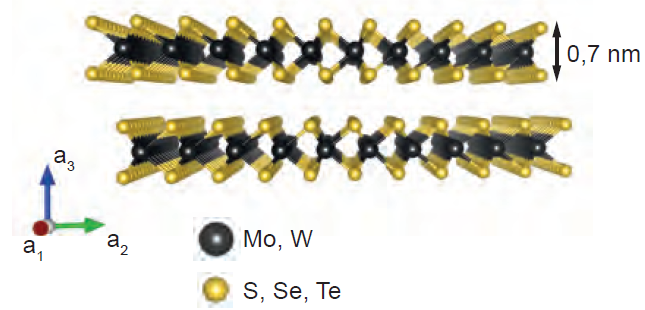
\includegraphics[width=\textwidth]{img/tmdc_structure.png}
    		\caption{}
    		\label{fig_tmdc_structure}
    \end{subfigure}
    \hfill
    \begin{subfigure}{0.37\textwidth}
        \centering
        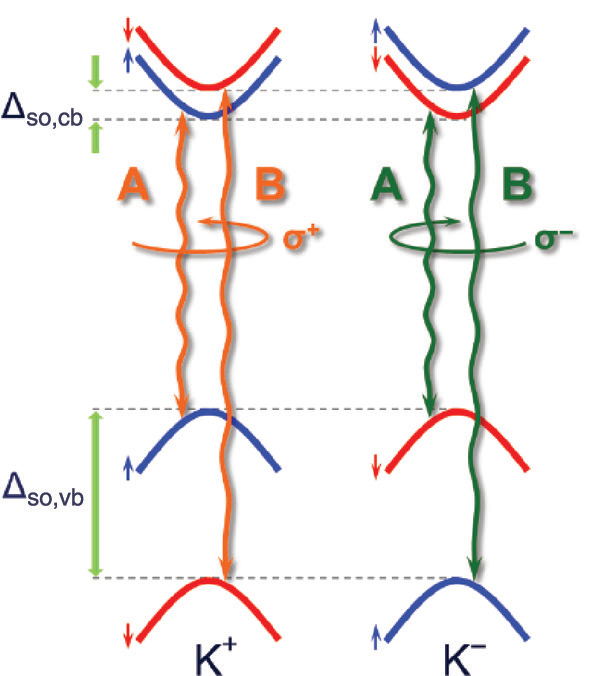
\includegraphics[width=\textwidth]{img/AB_exc.png}
        \caption{}
	      \label{fig_valley_split}
    \end{subfigure}
    \caption{a: Layered crystal structure of TMDCs. \cite{Schmidt2016}. b: Valley dependence on spin splitting in monolayer TMDCs.\cite{Koperski2017} }
	\label{fig_tmdcs} % 3->1
\end{figure}


\subsection{Single-photon emitters}
\label{sec:theory:spe}
%TODO Hanbury-Brown-Twiss

Single-photon emitters (SPEs) are light sources that don't emit more than one photon at once.
SPEs are identified by performing photon antibunching, meaning that two detectors are used, whith one giving a start signal and the other the stop signal, allowing the measurement of the so called second-order correlation function $g^{(2)}(\tau)$.
If the emitter in question is a Single-photon emitter, there will be a significant dip in the relative quantity of delays between start and stop signal close to zero.

\subsection{Magneto-optic effect}

	The interaction of electromagnetic waves with matter can be described with the refractive index
	\begin{align*}
		\tilde{n} = n + ik \,,
	\end{align*}
	where $n$ describes the refraction and $k$ the absorption.
	From this information on reflection and transmission can also be extracted.
	Adding an external magnetic field to the matter, changes its refractive index for different polarizations of the incoming electromagnetic wave.

  Linear polarized light can be described by a superposition of two circular polarized electromagnetic waves, one left- and one right-polarized.
	When passing through the matter, the left- and right-polarized parts change differently in intensity and phase.
	The result is that the superposition of both waves no longer adds to linear polarized, but elliptic polarized light.
	From the phase change results a rotation of the lights main oscillation axis and from the intensity change the ellipticity.
	This rotation is also known as Faraday rotation.
	Here, it should be noted that this is the case for transmission through matter.
  For reflection on the other hand a similiar effect, namely the magneto-optical Kerr effect, takes place.

	\

	As the change in polarization through interaction with magnetized matter is heavily dependent on the properties of the matter, band structure information can be obtained using magneto-optic methods.
	An example of this is given by spin polarized band gaps.
	For this investigation, the Zeeman-splitting for 1s-excitons in TMDCs and how they influence the refractive properties of matter is of interest.
	This can be described by the Verdet constant $V$ which is given by:
	\begin{align*}
		V = \frac{\varphi_\text{F}}{L\cdot B} \,,
	\end{align*}
	where $\varphi_\text{F}$ is the Faraday rotation, $L$ the thickness of the sample and $B$ the strength of the external magnetic field.

	To allow the deduction of the Faraday rotation by measurement of transmission intensities, Jones matrices can be used.
	They describe the change of polarization in the plane transverse to the light's direction of propagation.
	For example the sample can be described by
	\begin{align*}
		\hat{\text{S}} = \left( \begin{array}{rr}
		1 & (\varphi_\text{F} + i\eta_\text{F}) \\
		-(\varphi_\text{F} + i\eta_\text{F}) & 1 \\
	\end{array}\right) \,,
	\end{align*}
  with $\eta_\text{F}$ being the ellipticity of the polarization.
	The electric field of initially linearly polarized light $\hat{E}_i$ can be written as a two-component vector:
	\begin{align*}
		\hat{E}_i = \left( \begin{array}{r}
					\cos{p} \\
					\sin{p} \\
				\end{array}\right) \,,
	\end{align*}
	where $p$ describes the angle of the linear polarization.
	By multiplying this vector with the Jones matrices $\hat{J}_k$ of the different objects in the beams path, expressions for the measured intensities $T_i = E_i^* E_i$ can be calculated.
  Specifically, $E_i \propto \prod_k \hat{J}_k \cdot \hat{E}_i$.
  Here, the indices $i$ are assigned to the two components of the initially linear polarized light.

  The faraday rotation results from taking the difference of the measured intensities $T_i$ each divided by the intensities measured without a sample $T_i^0$:
	\begin{align*}
		\frac{T_1}{T_1^0} - \frac{T_2}{T_2^0} = 4 \varphi_\text{F} + \varphi_\text{bg} \,.
	\end{align*}
	Additionally, there is $\varphi_\text{bg}$, which amounts to noise expected to be measured without the sample.

	\section{Monolayers}
\label{sec:mono}

\subsection{Execution}

The following is conducted for two different unknown TMDCs:
Firstly the scotch tape technique is used, to separate the layers from a thick crystal.
These layers are then transferred to a gel strip, from which they are subsequently transferred onto a silicon wafer that has an SiO$_2$ layer on top.

In order to now find pieces on the wafer that are monolayers, an optical microscope is used, utilizing the fact that due to the different refractive indeces of Si, the SiO$_2$ and the deposited material different thicknesses appear in different colors \cite{benameur2011}.
The samples are then transferred to a widefield microscope, a schematic of which is shown in \cref{fig_widefield}.
%TODO da noch was beschreibendes zu
%TODO numerische Apertur von der Linse
Apart from also having imaging properties, a slit can be inserted into the widefield microscope, to record a spectrum using a basic light spectrometer.
Due to the insertion of the slit, imaging properties in one direction are lost in the process.

\begin{figure}[!ht]
    \centering
    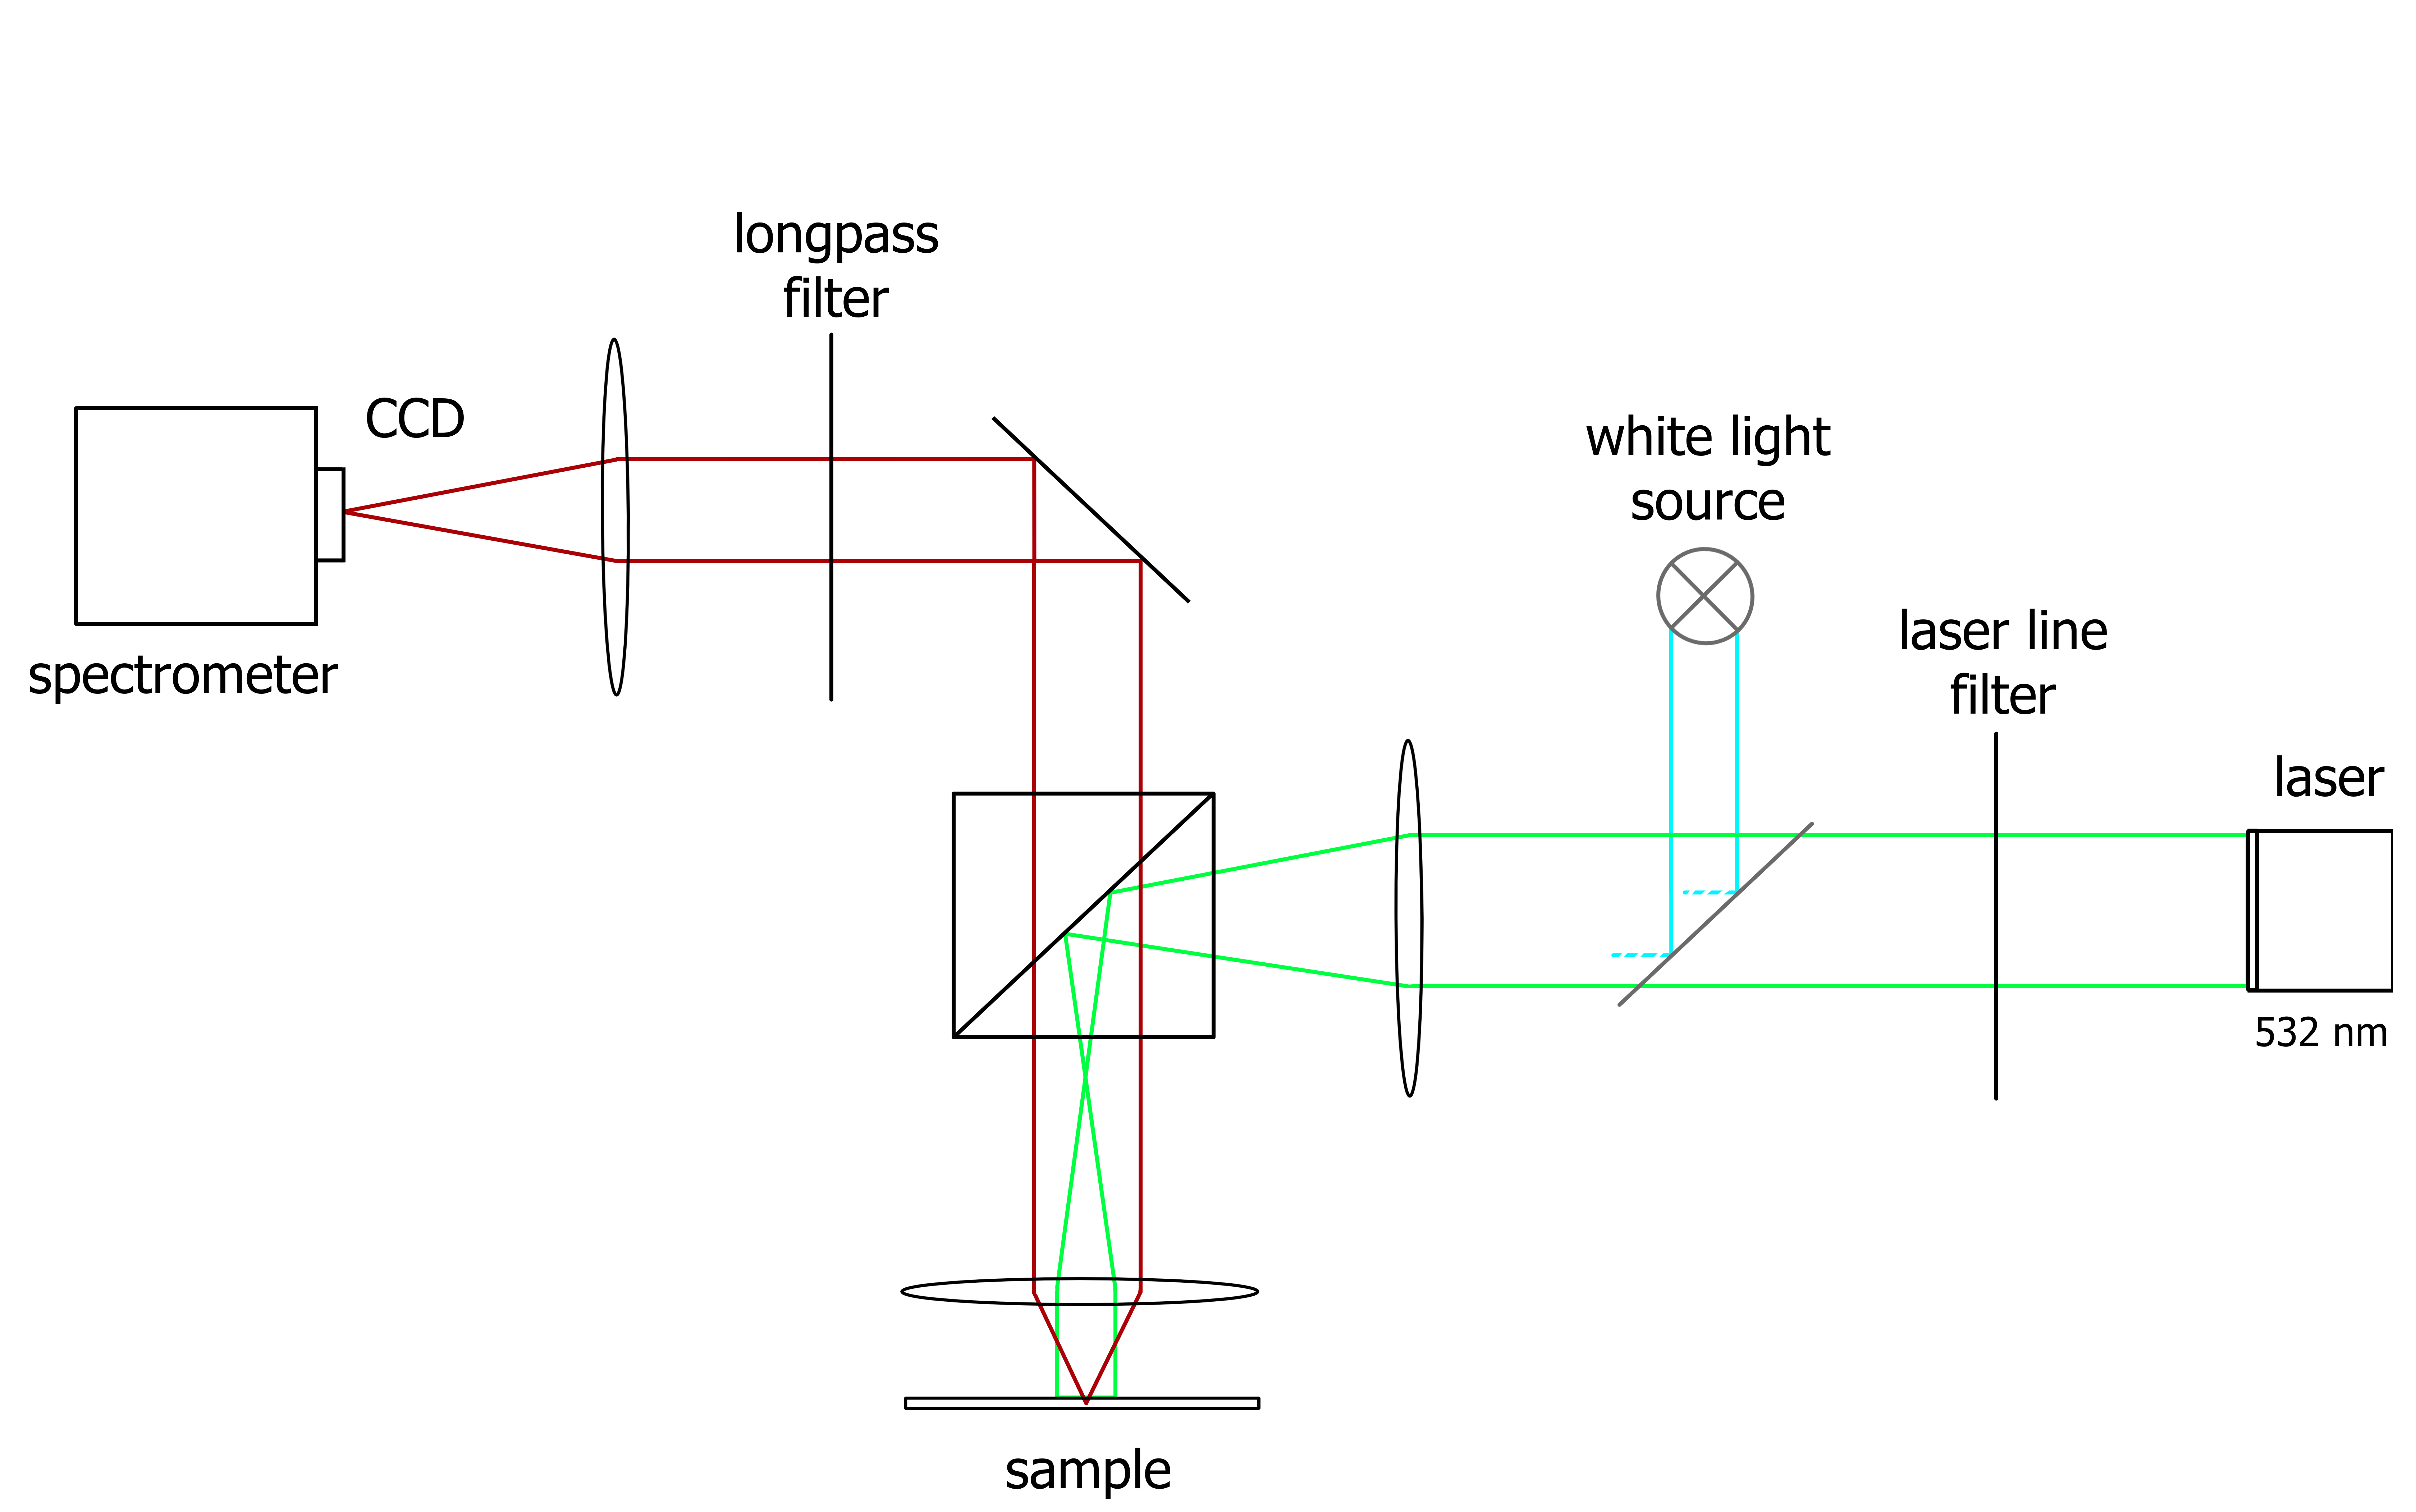
\includegraphics[width=0.7\textwidth]{img/setup1.png}
    \caption{Schematic of the widefield microscope used to record photoluminescence spectra. The detector corresponds to a spectrometer.}
    \label{fig_widefield}
\end{figure}


\subsection{Analysis}

	\section{Single-Photon Emitters}
\label{sec:SPE}
%Bei höheren Intensitäten sollte der Dip schmaler werde, weil dann der Emitter näher an Sättigung geht und zunehmend die Lebensdauer des angeregten Zustands statt der Einstrahlphotonenrate relevant ist
%Bei 2mW angefangen zu blinken. Spektrum trotzdem gut
%Für die Spektren gegen Wellenlänge die Fläche drunter integrieren und gegen Leistung plotten

\subsection{Execution}

\begin{figure}[H]
    \centering
    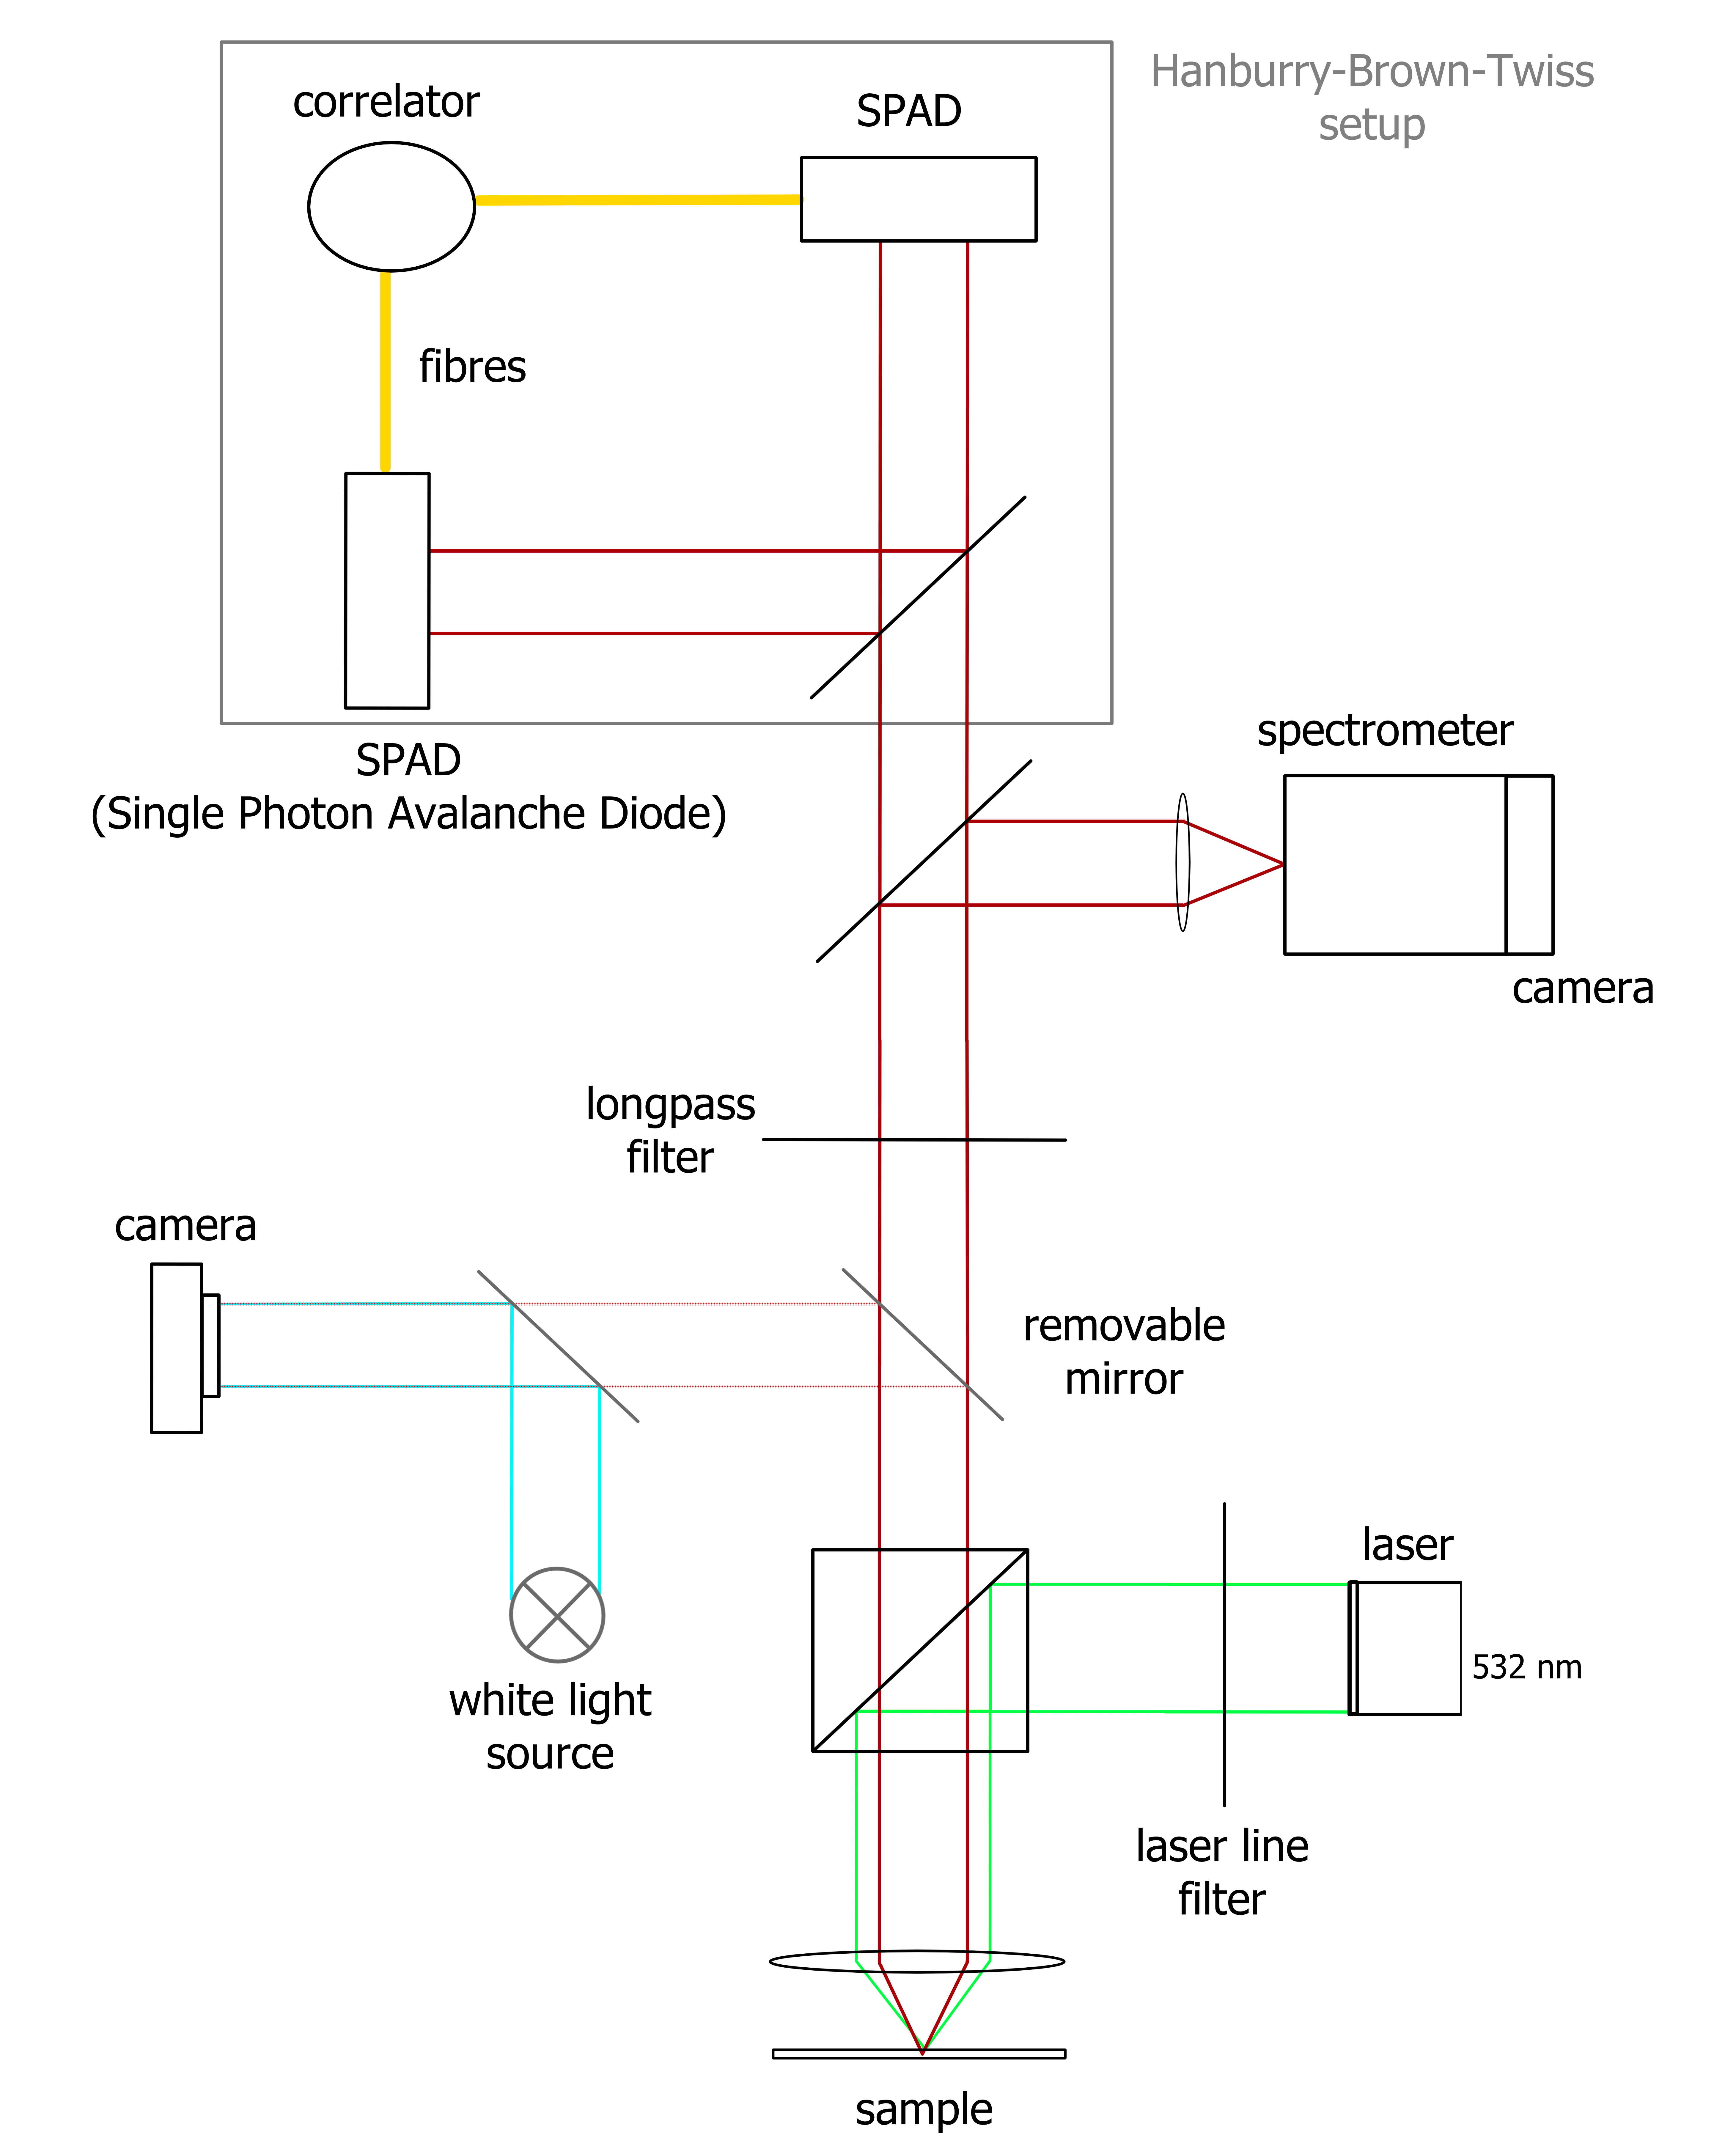
\includegraphics[width=0.6\textwidth]{img/setup2.png}
    \caption{Schematic of the confocal microscope used to record photoluminescence antibunching autocorrelation plots.}
    \label{fig_confocal}
\end{figure}

Hexagonal boron nitride powder on a substrate is viewed through a confocal microscope, which is shown in \cref{fig_confocal}.
In order to navigate on the sample, a white light source and a camera are used.
For the measurements a laser and a detector is used.
The laser is passed through a laser line filter, to sharpen its energy distribution.
The pinhole causes light not emitted from the desired plane to be excluded, allowing focusing along the optical axis.
% was ist jetzt der Sinn von dem pinhole? Eigentlich würde ich ja das mit dem aus einer Ebene sagen, aber er meinte ja irgendwas anderes.
Once a promising region is found, the laser and the detector (a spectrometer) are used, to record spectra at different spots on the sample, until a likely single photon emitter (SPE) is found.
The likely SPE is identified through having a clean spectrum that only contains peaks of one SPE and no other photon sources.

Once a suspected SPE is found, an antibunching measurement is conducted, by replacing the spectrometer with two fibres that split the light into two parts, that are seperately measured with two detectors as described in \cref{sec:theory:spe}.
These measurements are conducted for a series of different excitation laser powers and for each measurement a seperate background measurement is done, by sending the laser immediately onto the detector without passing the sample.

Additionally spectra are also recorded for increasing laser powers. %verwechsele ich laser powers oder ist das doppelt mit dem vorherigen Satz? ->ne, das davor bezieht sich auf Antibunching und hier meine ich die Spektren.

\subsection{Analysis}
\subsubsection{Antibunching}
\label{sec:spe:analysis:antibunch}

In \cref{fig_antibunch_raw} the raw measurement data recorded in the procedure described above is shown.
In the following the measurement of the SPE will be called $S(\tau)$ and the background measurement will be called $B(\tau)$ with $\tau$ the delay measured between the two detectors.
It can be seen, that peaks exist in both measurements.
These stem from resonances within the laser, causing a not completely constant photon output rate of the laser at this small timescale.
As these resonances are independent of the sample, the background measurement contains only these resonances and can be used to derive a background corrected signal $\tilde{S} (\tau)$.
If the average number of counts in a bin far away from the dip or any resonances is $I_S$ for the SPE measurement and $I_B$ for the background, the correction can be done as follows:
\begin{equation}
  \tilde{S} (\tau) = S - \frac{I_S}{I_B F} (B-I_B) = S - \frac{I_S}{I_B F} B + I_S
\end{equation}
Here $B-I_B$ gives only the resonance peaks and $\frac{I_S}{I_B}$ renormalizes them from the background measurement to the SPE measurement.
The factor $F$ is added artificially and is manually adjusted for each measurement, as without it the resonance peaks are overestimated causing minima in the corrected signal.
This may be due to the existence of the sample having an effect on the relative intensity of the peaks.
In order to do this the term $\frac{I_S}{I_B F} (B-I_B) + I_S$ is plotted in comparison to the uncorrected signal as shown in \cref{fig_antibunch_background_comp} and $F$ is adjusted, until the resonance peaks match up.
The values used for $F$ lie in the range of \SIrange{1,5}{6}{}.
In \cref{fig_antibunch_raw_corr_comp} the corrected signal $\tilde{S}$ is compared to the raw signal $S$.
Also the delay times are adjusted by an offset of \SI{98,5}{ns}, so that the dip lies at \SI{0}{ns}.
This is necessary due to slightly different travelling time of the signal between the detectors.
Only the part of the measurement close to the dip is shown.


\begin{figure}[H]
    \centering
    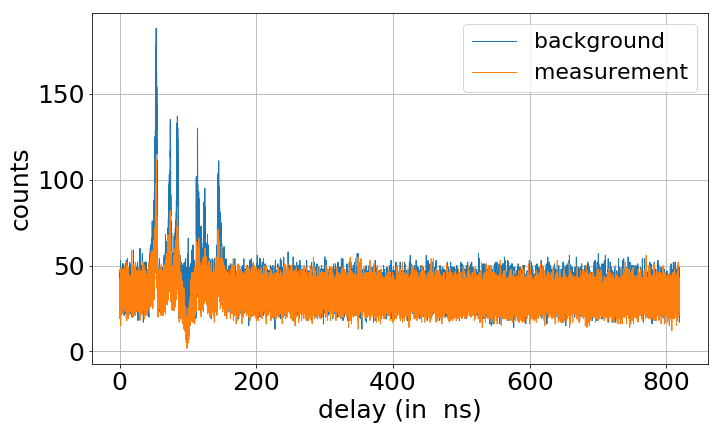
\includegraphics[width=0.7\textwidth]{img/output_t2/antibunch_example_50.0muW.png}
    \caption{Antibunching measurement of hBN and the background measurement as recorded for a laser power of \SI{50}{\micro W}.}
    \label{fig_antibunch_raw}
\end{figure}

\begin{figure}[H]
    \centering
    \begin{subfigure}{0.7\textwidth}
        \centering
        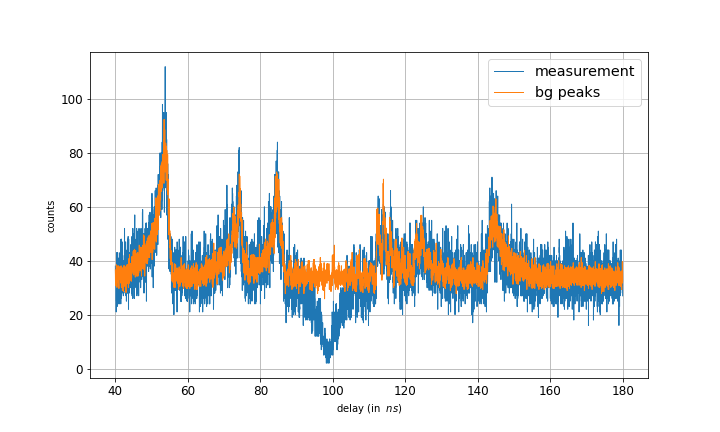
\includegraphics[width=1.0\textwidth]{img/output_t2/50.0muW_bg_peaks.png}
    \caption{}
    \label{fig_antibunch_background_comp}
    \end{subfigure}
    %\hfill
    \begin{subfigure}{0.7\textwidth}
        \centering
        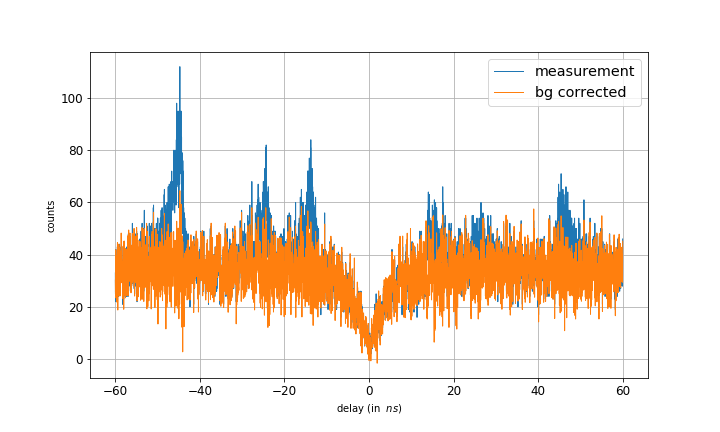
\includegraphics[width=\textwidth]{img/output_t2/50.0muW_bg_vgl.png}
        \caption{}
        \label{fig_antibunch_raw_corr_comp}
    \end{subfigure}
    \caption{a: Antibunching measurement as recorded and compared to the adjusted background signal. b: Antibunching measurement as recorded and compared to the background corrected signal. The laser power is \SI{50}{\micro W}.}
	\label{fig_antibunch_comp}
\end{figure}

This is done for six different powers and shown in \cref{sec:anhang:spe}.

These antibunching measurements show that indeed a single photon emitter was found, as they all show a significant dip at a delay between start and stop signal of \SI{0}, because this means that it is at least much less likely that the source emits two photons at once, than at a finite delay.
It can also be seen that for very high laser powers the edges of the signal start to decrease significantly with the absolute value of the delay time.
This can be explained by the fact, that here the photon rate emitted from the laser and thereby from the sample is so high that large delays between start and stop signal become increasingly unlikely independently of the sample.

In order to characterize the behavior of the source at increasing excitation powers, the depth of the dip and the width of the dip at half of its depth is manually read from the charts.
The results are shown in \cref{fig_dip_depth} and \cref{fig_dip_width}.
The depth is normalized by $I_S$ to ensure comparibilty between measurements.
The uncertainties are gauged from the thickness of the noise.
For the power an uncertainty of $1\%$ is assumed.

\begin{figure}[H]
    \centering
    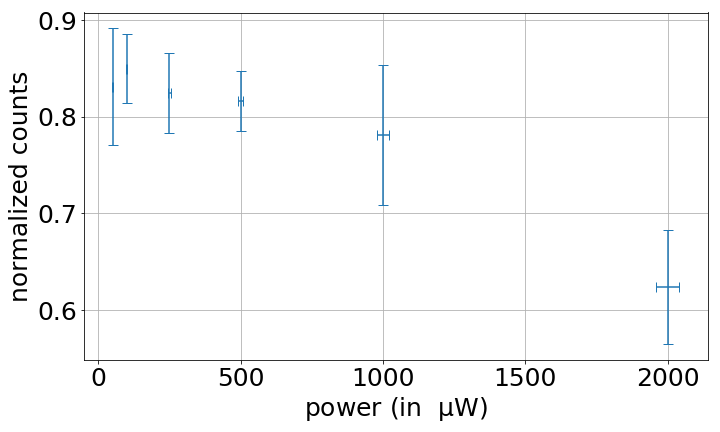
\includegraphics[width=0.7\textwidth]{img/output_t2/dip_depth.png}
    \caption{Depth of the dips in the antibunching measurements plotted against the laser power.}
    \label{fig_dip_depth}
\end{figure}

\begin{figure}[H]
    \centering
    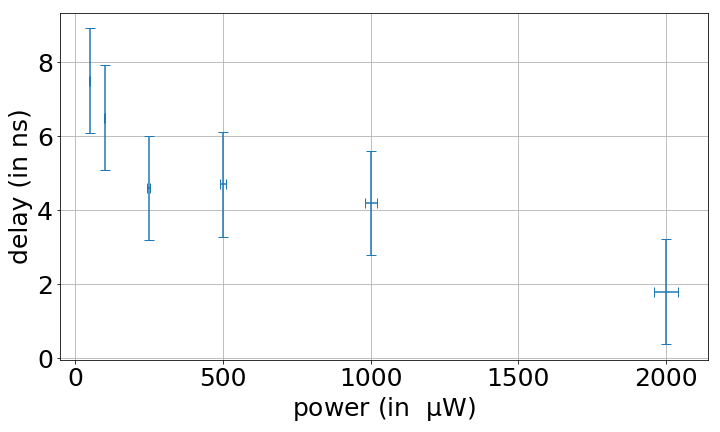
\includegraphics[width=0.7\textwidth]{img/output_t2/dip_width.png}
    \caption{Width of the dips in the antibunching measurements plotted against the laser power.}
    \label{fig_dip_width}
\end{figure}

It can be seen that both the depth and the width decreases with increasing laser power.
For the depth this can only be explained by the increasing likelyhood that two photons hit the detectors at the same time, with at least one of them not stemming from the SPE (e.g. a reflection).
But as the width decreases at the same time, it can be seen that the emitter doesn't reach complete saturation, as in this case only the constant background would increase, causing the width at half depth to increase as well.
% jetzt wo ich das geschrieben habe, finde ich diese beiden Plots nicht sehr aussagevoll, da das beides ziemlich obvious ist, aber ich weiß nicht, was ich sonst mit den ganzen antibunching messungen machen soll.

It is also observed that the SPE starts blinking at high powers, disappearing for short periods of time, before reappearing.
This can be explained, by supposing that at this photon rate the emitter reaches periods of saturation in the way that electron-hole pairs are created faster than they can decay, causing periods of time, where there are no excitable electrons available.

\subsubsection{Spectra and Power efficiency of the SPE}

In \cref{fig_spe_spectrum_example} an example of the recorded spectra is shown.
A constant background has been substracted, so that there are no counts at high wavelengths.
The large peak corresponds to the main zero-phonon decay of an exciton, while to the right two peaks of the one-phonon decay and even two very small peaks of the two-phonon decay can be seen.
For the one-phonon decay one peak belongs to longitudinal phonons and one to transverse phonons.
Though for the two-phonon decay three combinations are possible (longitudinal-longitudinal, longitudinal-transverse, transverse-transverse), only two small peaks can be seen in the spectrum, possibly because the energy difference between two of these combinations doesn't exist or isn't high enough to allow seperation at these low count rates.
%vmtl optisch, aber kp
The small peak at \SI{532}{nm} is caused by the reflection of the laser itself, as this is its wavelength.
It is small, because most of it gets filtered out by the longpass filter.

\begin{figure}[H]
    \centering
    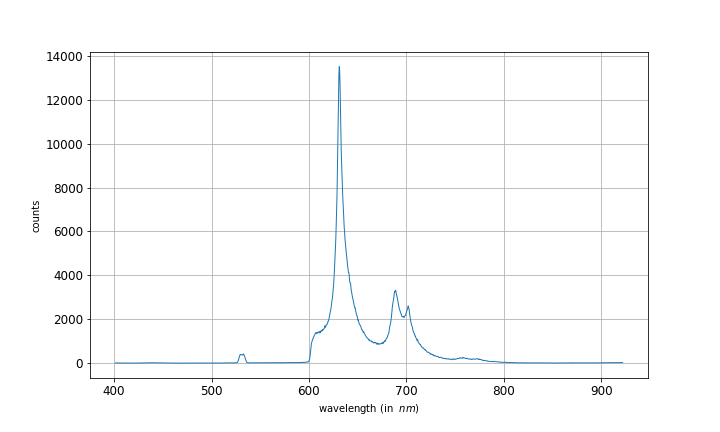
\includegraphics[width=0.7\textwidth]{img/output_t2/spektrum_example_bgcorr_200.0muW.png}
    \caption{Recorded Spectrum of the observed single photon emitter at a laser power of \SI{200}{\micro W}. A constant background has been substracted.}
    \label{fig_spe_spectrum_example}
\end{figure}

In order to observe the behavior of the SPE at increasing laser powers, in \cref{fig_spe_integrals} each spectrum has been integrated and normalized over the time that the spectrum was recorded over. %theoretisch hätte man hier den Laserpeak rauslassen sollen, aber macht auch keinen großen Unterschied.
It can be seen, that the output increases mostly linearly with the power meaning that the efficiency is approximately constant.
It would be expected that at higher powers the SPE approaches saturation, causing the efficiency to go down and the increase in output photons to be reduced.
This could not be seen, as the observed SPE died at \SI{450}{\micro W}.
%warum nicht linear bei kleinen Leistungen?

\begin{figure}[H]
    \centering
    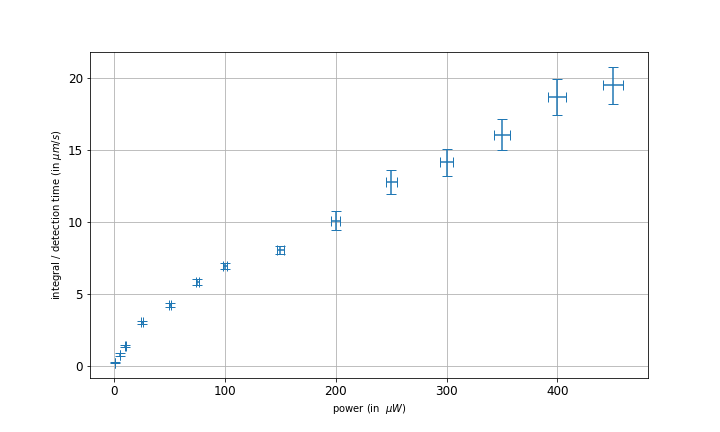
\includegraphics[width=0.7\textwidth]{img/output_t2/integrals.png}
    \caption{Integrated spectra of the SPE normalized by the detection time at different laser powers.}
    \label{fig_spe_integrals}
\end{figure}

	\newpage
\section{Faraday Rotation}

\subsection{Execution}

\begin{figure}[!ht]
    \centering
    \includegraphics[width=0.85\textwidth]{img/setup3.png}
    \caption{Schematic of the setup used to record faraday rotation. As sample a WS$_2$ monolayer is used.}
    \label{fig_setup3}
\end{figure}
To measure the Faraday rotation of a WS$_2$ monolayer a novel setup by Dr. Ashish Arora and Dr. Benjamin Carey is used.
It is presented in \cref{fig_setup3} and allows a much faster acquisition of a whole spectrum than with previously used methods.
Here, two types of illumination ares used.
Firstly a laser to excite the monolayer and secondly a white light source to cover a broad energy spectrum rather than one energy at a time.
After polarizing the beam, it travels through the sample inside a magnetic field.
The transmitted light is then deflected into a lens system for reducing noise and focussing.
A key component in this setup is the beam displacer, where the beam splits into two.
This is dependent on the change in polarization induced by the sample.
Both beams are then each focused on a row on the CCD-chip, which acts as a spectrometer.
Again, to reduce noise the signals around the chosen rows are taken and subtracted as background.

\

According to the theoretical description in \cref{sec:theory}, measuring at a certain initial beam polarization allows us to obtain the Faraday rotation, however with background.
As this background does not change with the polarization, measurements are taken at \SI{+45}{\degree} and \SI{-45}{\degree} and then subtracted, since the Faraday rotation changes sign.

To ensure that the WS$_2$ monolayer is flat on a sapphire substrate, it is trapped between hexagonal boron nitride, which only adds a negligible contribution to the measured data.
Since the beam passes through both, the sapphire substrate and the WS$_2$ monolayer, again two measurements have to be taken do differentiate the background from the monolayer.
This is done by comparing the verdet constants of monolayer with substrate and of only substrate.

\subsection{Analysis}

\begin{figure}[!ht]
    \centering
    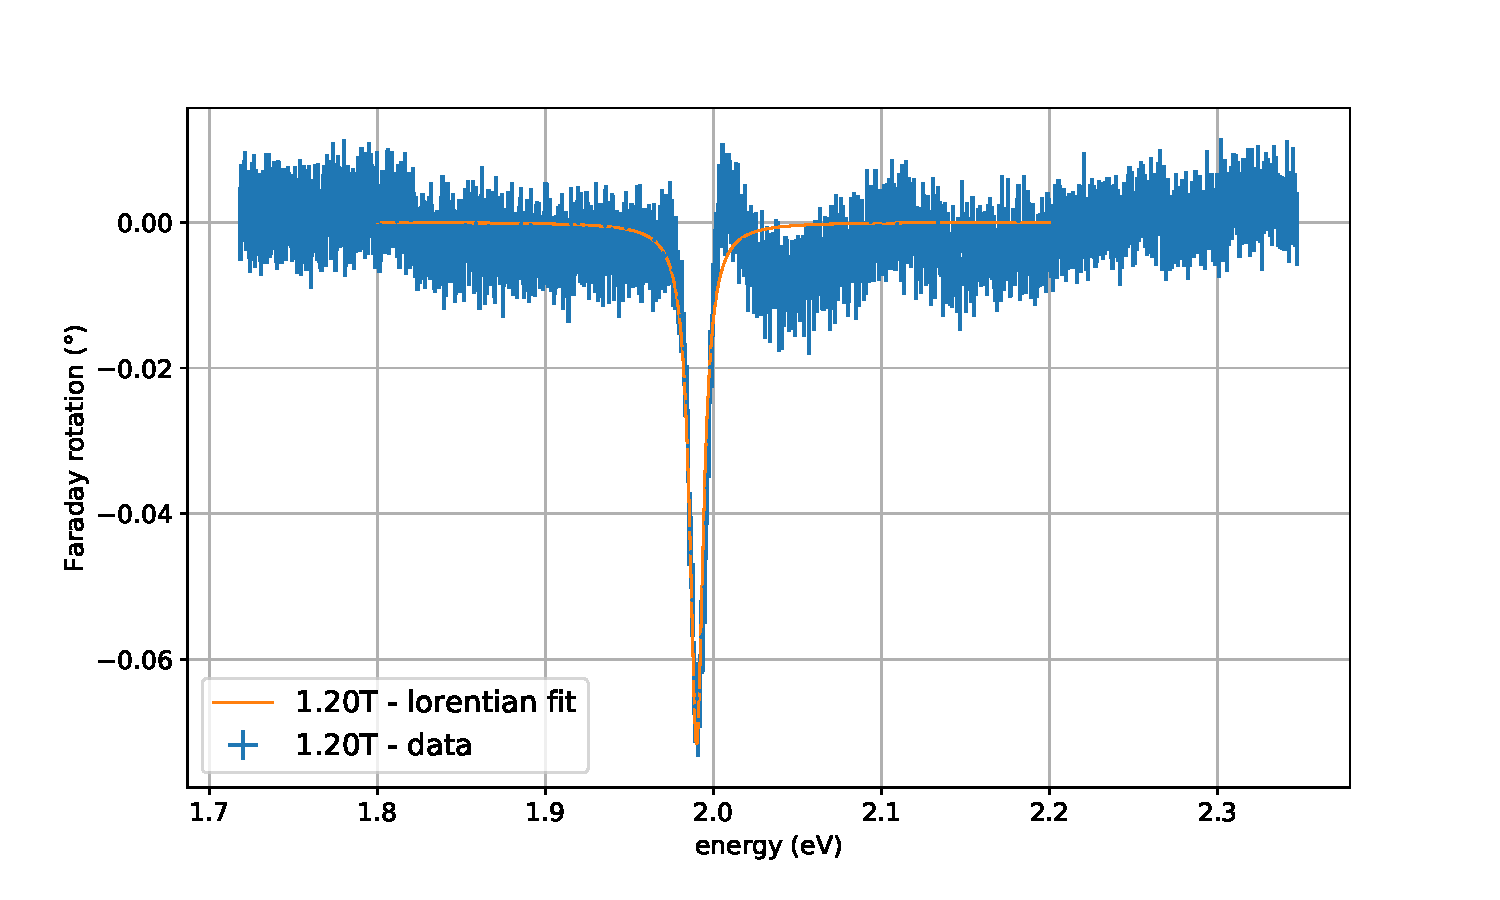
\includegraphics[width=0.85\textwidth]{plots/WS2_1200mT.pdf}
    \caption{Representation of WS$_2$ monolayer data points of the faraday rotation with external magnetic field of \SI{1.2}{\tesla} and lorentian fit.}
    \label{fig_WS2_1200mT}
\end{figure}
Since a lorentian line in the absorption spectrum is to be expected, lorentian fits are used for the data of the WS$_2$ monolayer.
An example is given in \cref{fig_WS2_1200mT} at \SI{1.2}{\tesla}.
All other plots of the data and their corresponding lorentian fits can be found in \cref{sec:appendix}.
Most of them fit very well with the data points, neglecting the noise.


\begin{figure}[!ht]
    \centering
    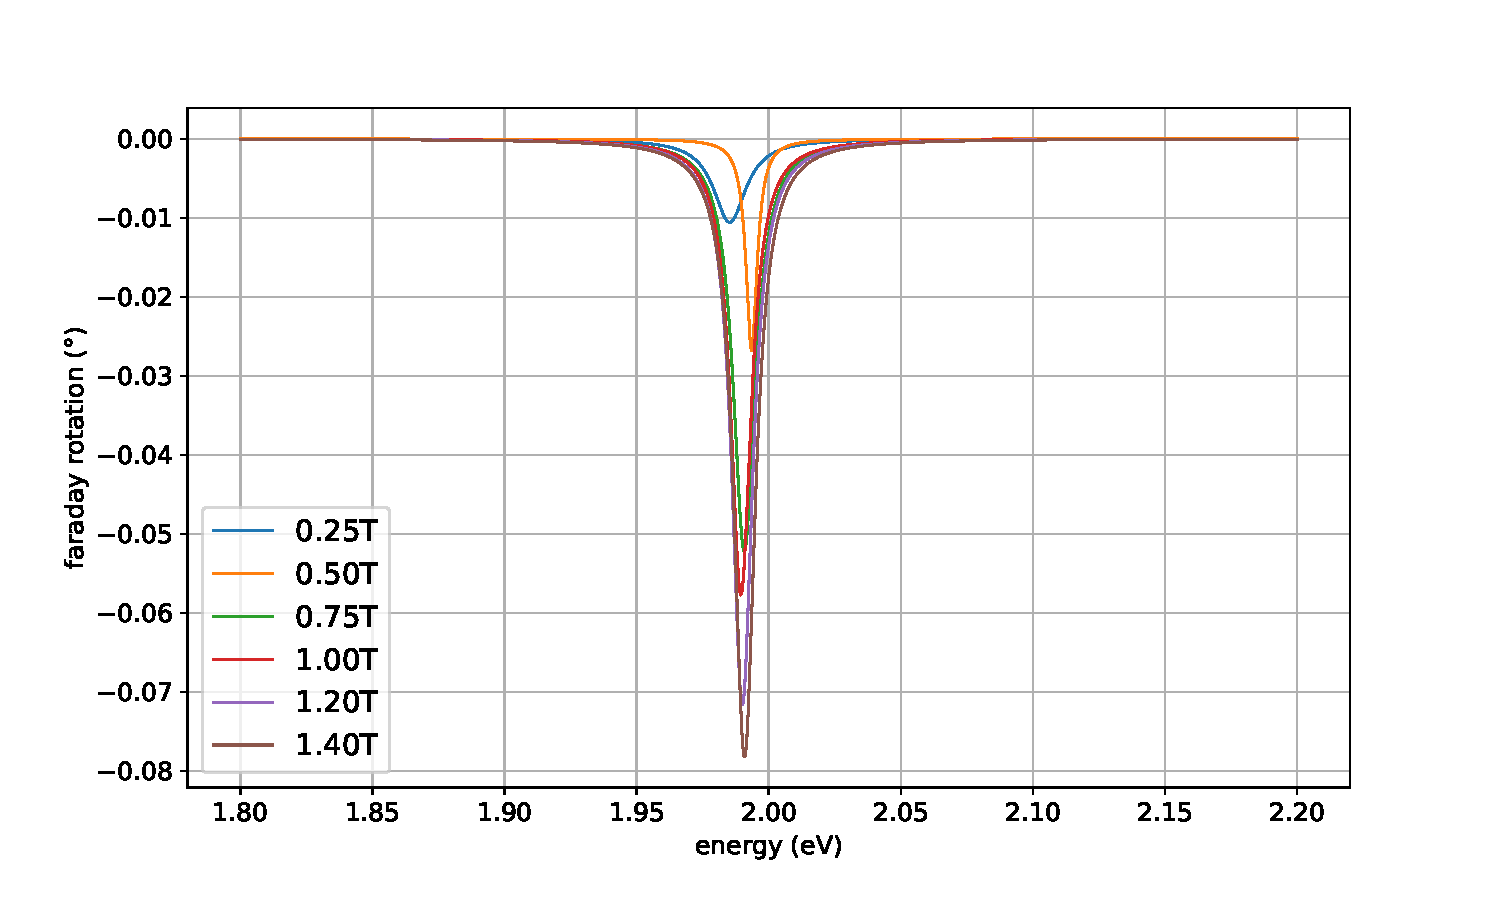
\includegraphics[width=0.85\textwidth]{plots/WS2_lorentians.pdf}
    \caption{Representation of all lorentian fits plotted together.}
    \label{fig_WS2_lorentians}
\end{figure}
For comparison all lorentian fits are found in \cref{fig_WS2_lorentians}.
As suspected an almost linear decrease is seen at the minima.
Only the minimum at \SI{0.75}{\tesla} does not fit very well.
This may be due to remanent magnetisation, as the spectra were not taken in order of rising magnetic field strength.
Also, the energy of the minima is not exactly the same for all magnetic field strengths, as it should be.
However, since they are almost the same the mean value of \SI{}{} gives a good estimate. % TODO

\begin{figure}[!ht]
    \centering
    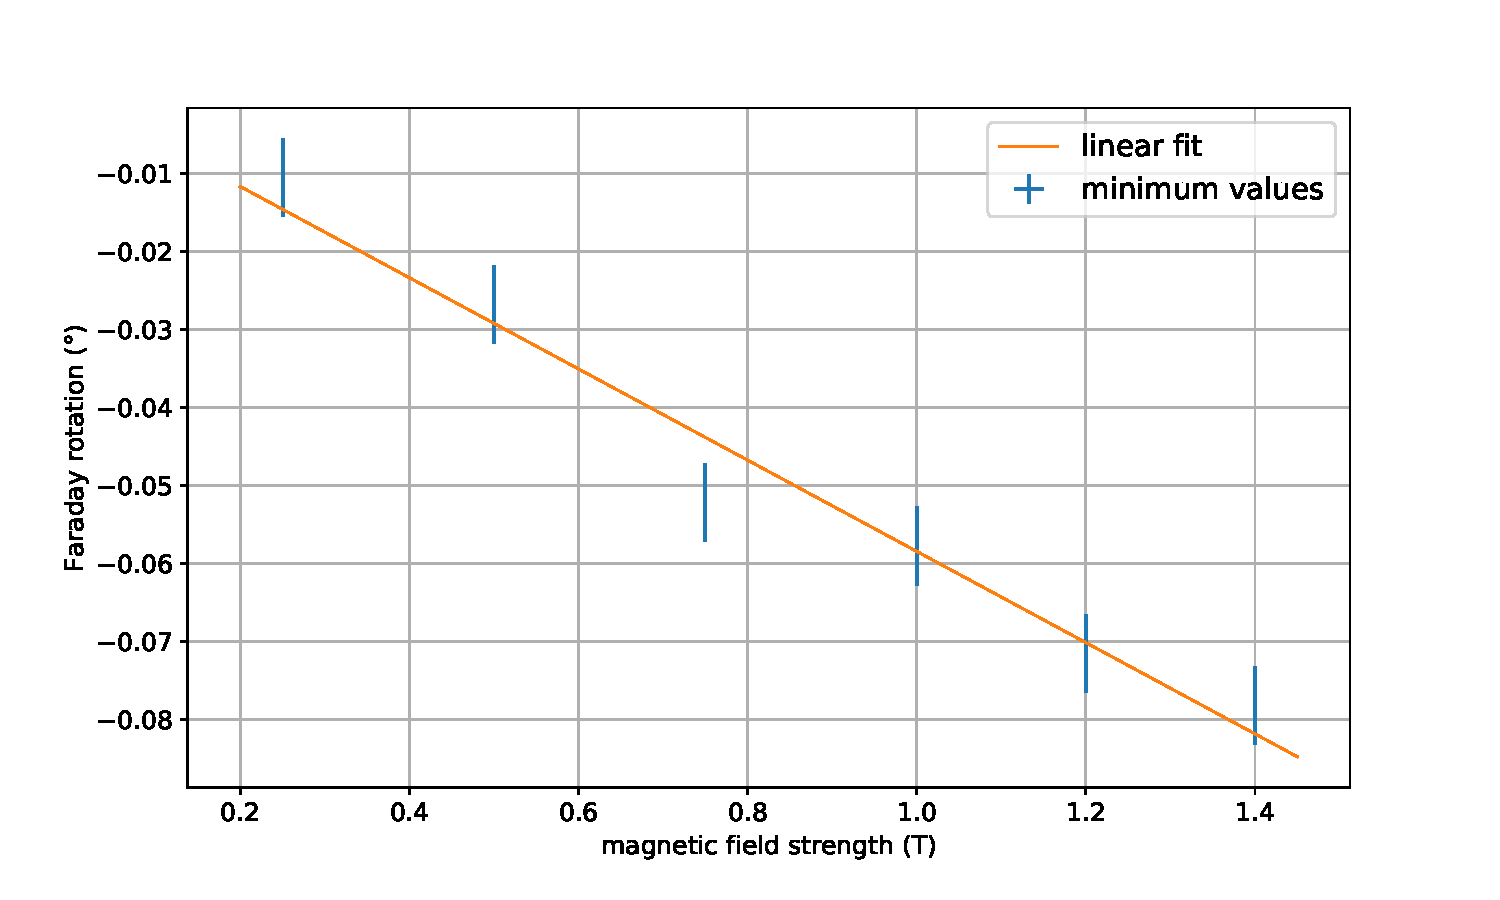
\includegraphics[width=0.85\textwidth]{plots/WS2_mins.pdf}
    \caption{Representation of largest WS$_2$s faraday rotation in dependence of external magnetic field strength.}
    \label{fig_WS2_minima}
\end{figure}
\cref{fig_WS2_minima} shows the beforementioned linear decrease by plotting the minima against the magnetic field strength.
Here, it also shows that the minimum at \SI{0.75}{\tesla} is a little of the expected value-

From its slope the verdet constant is extracted by division of the monolayers thickness of \SI{0.65}{\nano\meter}.
It amounts to \SI{}{}. % TODO

\

\begin{figure}[!ht]
    \centering
    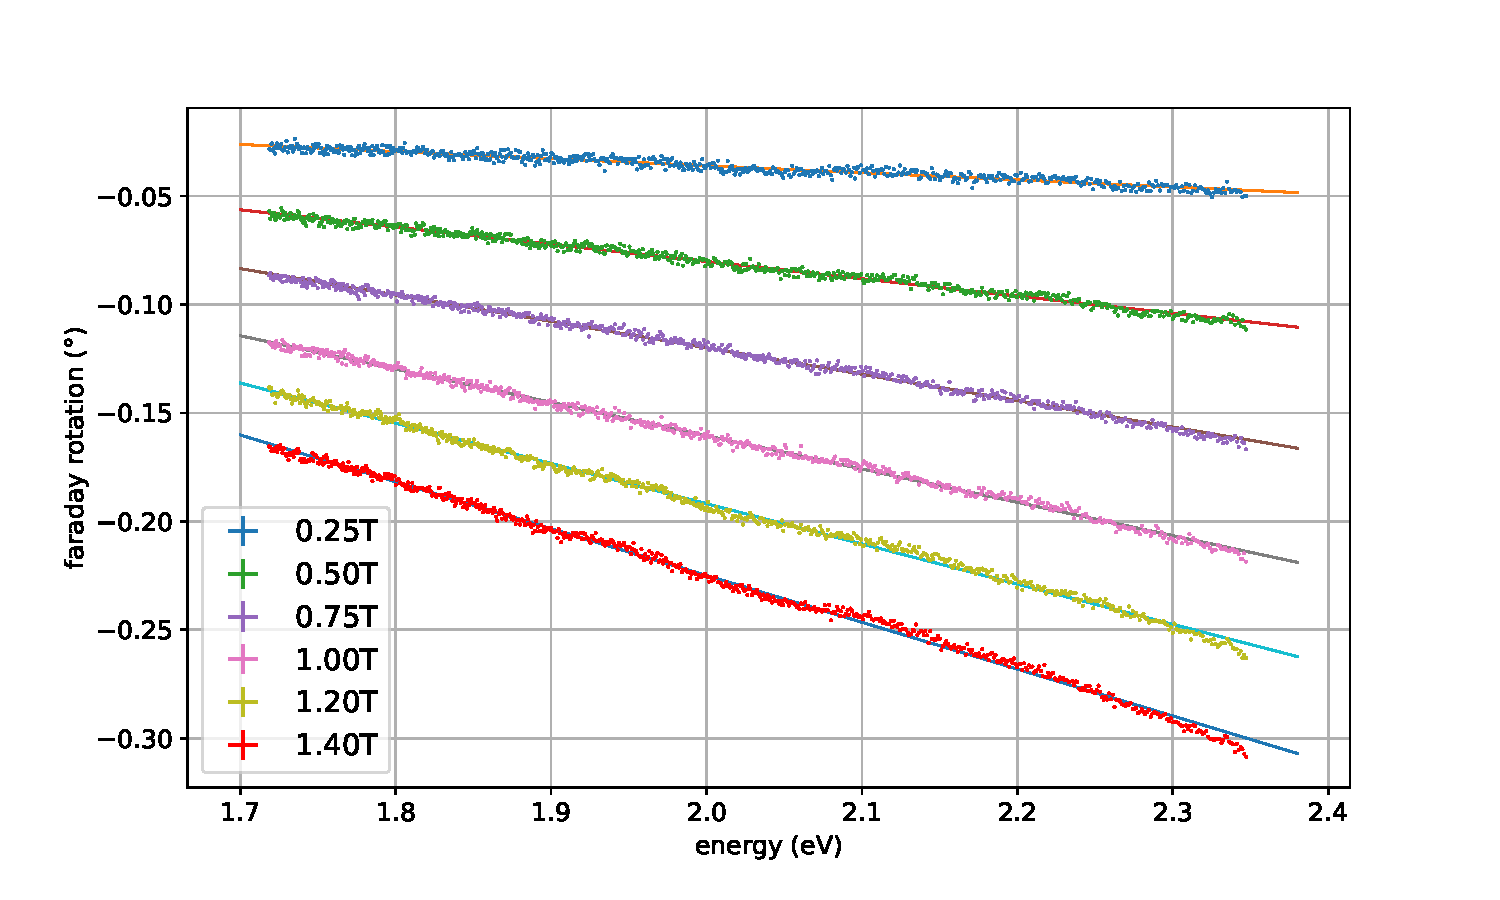
\includegraphics[width=0.85\textwidth]{plots/sapphire_lins.pdf}
    \caption{Representation of sapphire data points of the faraday rotation with different external magnetic fields and linear fits.}
    \label{fig_sapphire_lins}
\end{figure}
Contrary to the exciton contribution, only a linear decrease with rising energy is seen for the sapphire substrate in \cref{fig_sapphire_slopes}.
This linear decrease is fitted for each value of magnetic field strength.
The comparison of their slopes yet again shows another linear behavior.

\begin{figure}[!ht]
    \centering
    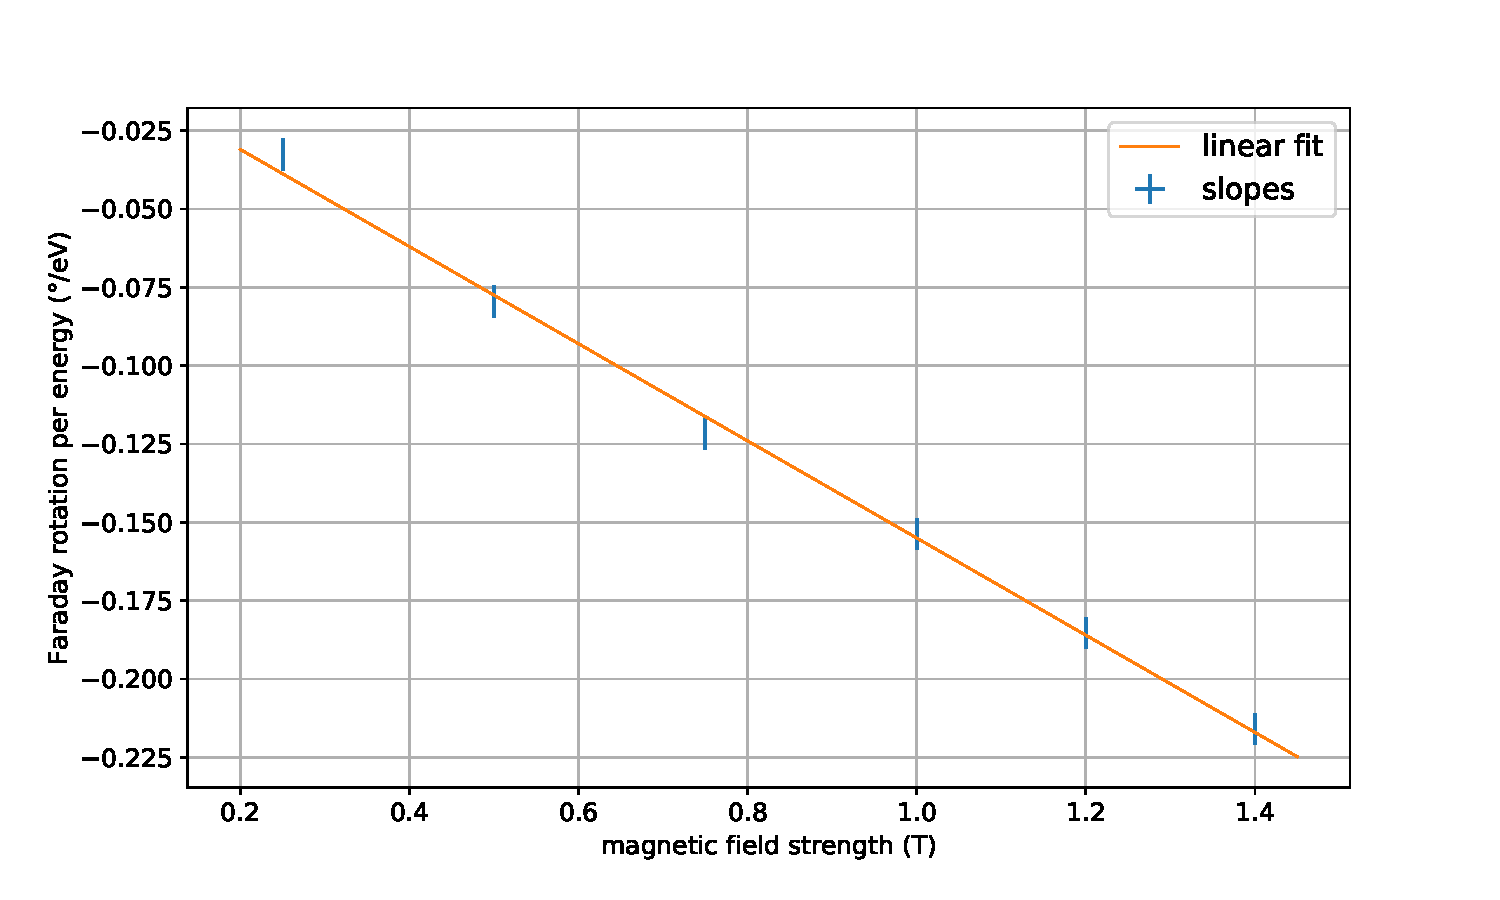
\includegraphics[width=0.85\textwidth]{plots/sapphire_slopes.pdf}
    \caption{Representation of sapphires faraday rotation in dependence of energy and external magnetic field strength.}
    \label{fig_sapphire_slopes}
\end{figure}
In \cref{fig_sapphire_lins} this is also fitted linearly.
Again by dividing this slope by the substrates thickness of \SI{0.5}{\milli\meter} the now energy dependent verdet constant of \SI{}{} is acquired.

To compare this value with the \SI{}{} of the WS$_2$ monolayer, it is multiplied with the energy of the minima and results in \SI{}{}.
These values differ in five orders of magnitude and thus show how strongly excitons influence the faraday rotation.

	% Bezug/Nutzen oder sonst was
	% auch hier die Hypothese wiederholen
	% keine Messwerte hier, nach manchen Menschen, zumindest "direkt" erstellte Diagramme net hier, auch wenn Lesbarkeit-bla
	\newpage
\section{Conclusion}
	% Rückgriff auf Hypothese und drittes Nennen dieser
	% Quellen zitieren, Websiten mit Zugriffsdatum
	% Verweise auf das Laborbuch (sind erlaubt)
	% Tabelle + Bilder mit Beschriftung

  % monolagen gefunden, Materialien konnten identifiziert werden (MoSe2 aber etwas unpassend)
  % SPE gefunden, Sättigung in Leistungsspektrum leider nicht

  In conclusion it can be said that it was possible to create monolayers of TMDCs using exfoliation and the materials used were identified within reasonable certainty by their respective exciton transition energy, though some deviation remained.

  It was also possible to find a single-photon emitter in a sample of hexagonal boron nitride by conducting antibunching measurements and the behavior of the emitter was quantified in dependence of incident laser power.
  The measurement of the efficiency of the emitter was incomplete, as the emitter didn't survive the measurement process.
  In the future it might be possible to reduce stress on the sample, by not performing several antibunching measurements of the same emitter at high laser powers, before measuring spectra.

  Lastly, the results regarding the faraday rotation are satisfying. It was possible to show the effect excitons have on the faraday rotation, as the corresponding Verdet constants were five orders of magnitude above those for an insulator like sapphire.

		% --- Anhang einbinden
	\newpage
\appendix
\section{Appendix}\label{sec:appendix}

\subsection{Uncertainties}\label{sec:uncertainties}

Any uncertainties will be calculated in accordance with GUM.
The equations used for that are seen in (\ref{fig:GUM_combine}) and (\ref{fig:GUM_formula}).
For the calculations the python library "uncertainties" will be used, which follows the guidelines of GUM.
As for the uncertainties of specific parameters the approximation curves of the $y$-uncertainties of those parameters will be regarded and the method of least squares used.
Here the method "scipy.optimize.curve\_fit()" from the uncertainties library is taken.

\begin{figure}[ht]
	\begin{equation*}
	x = \sum_{i=1}^{N} x_i
	;\quad
	\sigma_x = \sqrt{\sum_{i = 1}^{N} \sigma_{x_i}^2}
	\end{equation*}
	\caption{Formel für kombinierte Unsicherheiten des selben Typs nach GUM.}
	\label{fig:GUM_combine}
\end{figure}

\begin{figure}[ht]
	\begin{align*}
	f = f(x_1, \dots , x_N)
	;\quad
	\sigma_f = \sqrt{\sum_{i = 1}^{N}\left(\pdv{f}{x_i} \sigma_{x_i}\right) ^2}
	\end{align*}
	\caption{Formel für sich fortpflanzende Unsicherheiten erster Ordnung nach GUM.}
	\label{fig:GUM_formula}
\end{figure}

%\newpage
%\subsection{weitere Abbildungen}

\newpage
\subsection{SPEs additional figures}
\label{sec:anhang:spe}

\begin{figure}[H]
    \centering
    \begin{subfigure}{0.47\textwidth}
        \centering
        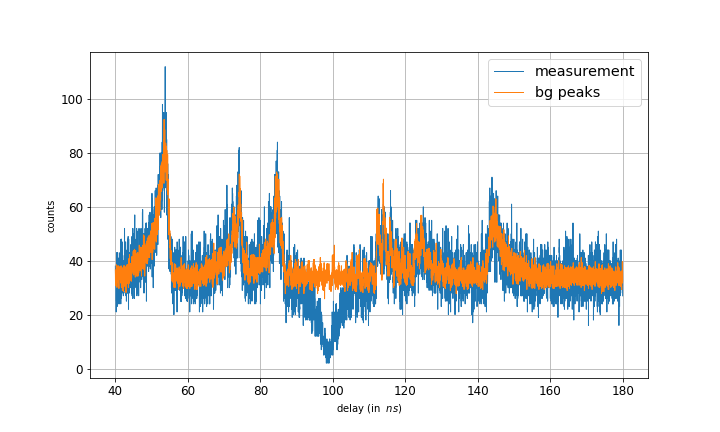
\includegraphics[width=1.0\textwidth]{img/output_t2/50.0muW_bg_peaks.png}
    		\caption{}
    		%\label{fig_antibunch_background_comp}
    \end{subfigure}
    %\hfill
    \begin{subfigure}{0.47\textwidth}
        \centering
        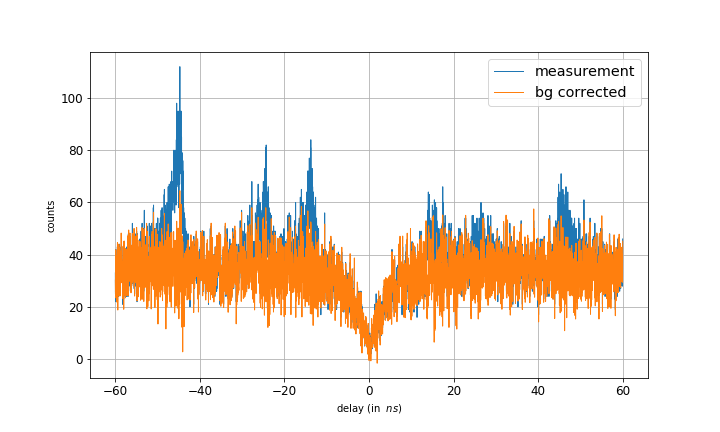
\includegraphics[width=\textwidth]{img/output_t2/50.0muW_bg_vgl.png}
        \caption{}
        %\label{fig_antibunch_raw_corr_comp}
    \end{subfigure}
    \caption{a: Antibunching measurement as recorded and compared to the adjusted background signal. b: Antibunching measurement as recorded and compared to the background corrected signal. The laser power is \SI{50}{\micro W}.} %hoffe ok, dass der eine so doppelt ist
	%\label{fig_antibunch_comp}
\end{figure}
\begin{figure}[H]
    \centering
    \begin{subfigure}{0.47\textwidth}
        \centering
        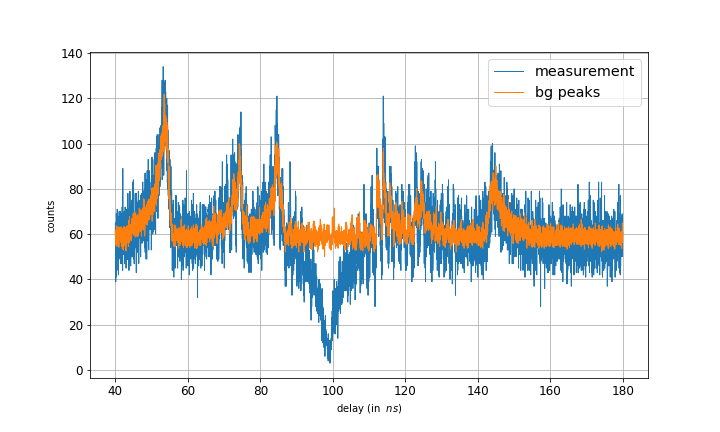
\includegraphics[width=1.0\textwidth]{img/output_t2/100.0muW_bg_peaks.png}
    \caption{}
    %label{fig_antibunch_background_comp}
    \end{subfigure}
    %\hfill
    \begin{subfigure}{0.47\textwidth}
        \centering
        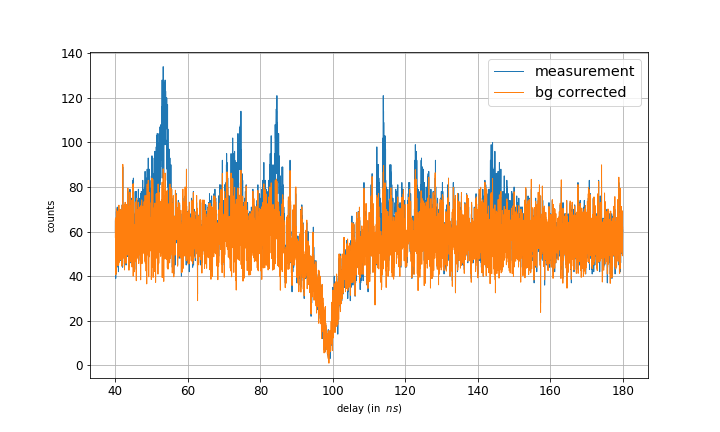
\includegraphics[width=\textwidth]{img/output_t2/100.0muW_bg_vgl.png}
        \caption{}
        %label{fig_antibunch_raw_corr_comp}
    \end{subfigure}
    \caption{a: Antibunching measurement as recorded and compared to the adjusted background signal. b: Antibunching measurement as recorded and compared to the background corrected signal. The laser power is \SI{100}{\micro W}.} %hoffe ok, dass der eine so doppelt ist
	%label{fig_antibunch_comp}
\end{figure}
\begin{figure}[H]
    \centering
    \begin{subfigure}{0.47\textwidth}
        \centering
        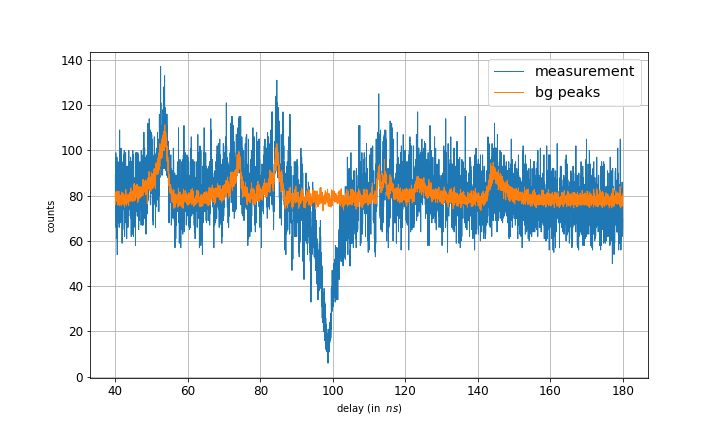
\includegraphics[width=1.0\textwidth]{img/output_t2/250.0muW_bg_peaks.png}
    \caption{}
    %label{fig_antibunch_background_comp}
    \end{subfigure}
    %\hfill
    \begin{subfigure}{0.47\textwidth}
        \centering
        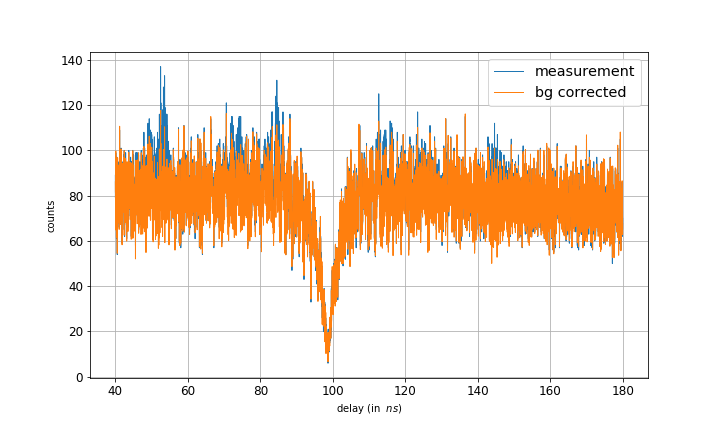
\includegraphics[width=\textwidth]{img/output_t2/250.0muW_bg_vgl.png}
        \caption{}
        %label{fig_antibunch_raw_corr_comp}
    \end{subfigure}
    \caption{a: Antibunching measurement as recorded and compared to the adjusted background signal. b: Antibunching measurement as recorded and compared to the background corrected signal. The laser power is \SI{250}{\micro W}.} %hoffe ok, dass der eine so doppelt ist
	%label{fig_antibunch_comp}
\end{figure}
\begin{figure}[H]
    \centering
    \begin{subfigure}{0.47\textwidth}
        \centering
        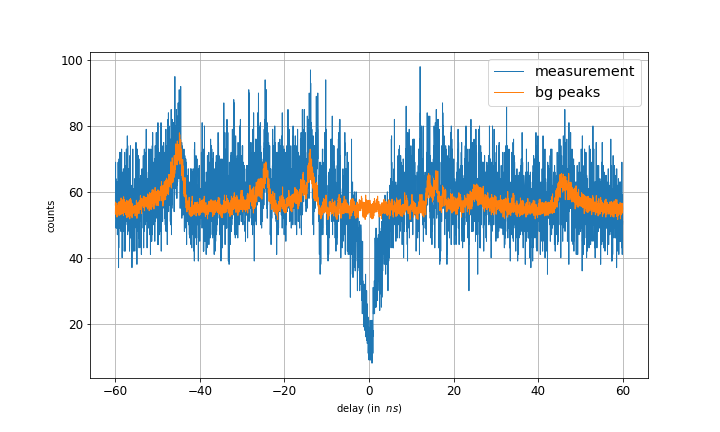
\includegraphics[width=1.0\textwidth]{img/output_t2/500.0muW_bg_peaks.png}
    \caption{}
    %label{fig_antibunch_background_comp}
    \end{subfigure}
    %\hfill
    \begin{subfigure}{0.47\textwidth}
        \centering
        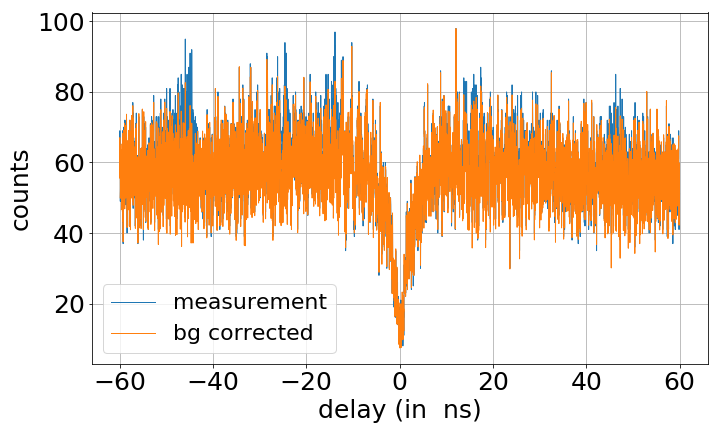
\includegraphics[width=\textwidth]{img/output_t2/500.0muW_bg_vgl.png}
        \caption{}
        %label{fig_antibunch_raw_corr_comp}
    \end{subfigure}
    \caption{a: Antibunching measurement as recorded and compared to the adjusted background signal. b: Antibunching measurement as recorded and compared to the background corrected signal. The laser power is \SI{500}{\micro W}.} %hoffe ok, dass der eine so doppelt ist
	%label{fig_antibunch_comp}
\end{figure}
\begin{figure}[H]
    \centering
    \begin{subfigure}{0.47\textwidth}
        \centering
        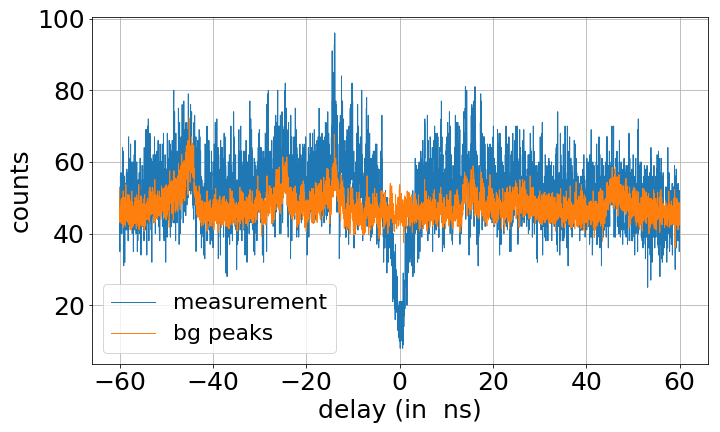
\includegraphics[width=1.0\textwidth]{img/output_t2/1000.0muW_bg_peaks.png}
    \caption{}
    %label{fig_antibunch_background_comp}
    \end{subfigure}
    %\hfill
    \begin{subfigure}{0.47\textwidth}
        \centering
        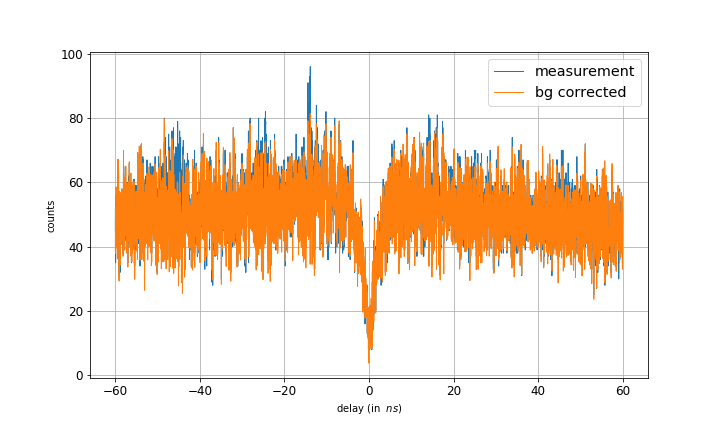
\includegraphics[width=\textwidth]{img/output_t2/1000.0muW_bg_vgl.png}
        \caption{}
        %label{fig_antibunch_raw_corr_comp}
    \end{subfigure}
    \caption{a: Antibunching measurement as recorded and compared to the adjusted background signal. b: Antibunching measurement as recorded and compared to the background corrected signal. The laser power is \SI{1000}{\micro W}.} %hoffe ok, dass der eine so doppelt ist
	%label{fig_antibunch_comp}
\end{figure}
\begin{figure}[H]
    \centering
    \begin{subfigure}{0.47\textwidth}
        \centering
        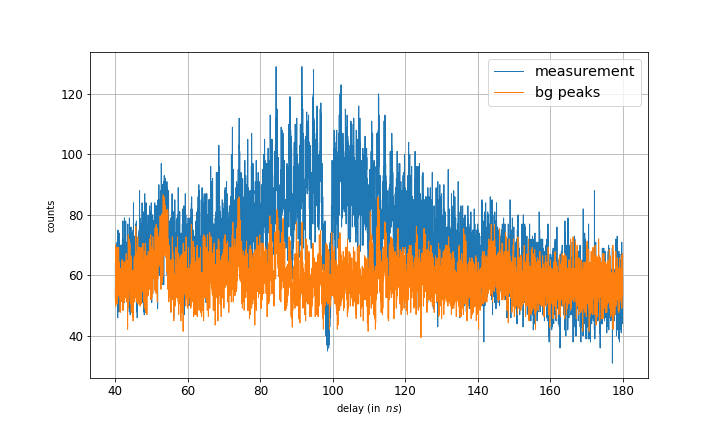
\includegraphics[width=1.0\textwidth]{img/output_t2/2000.0muW_bg_peaks.png}
    \caption{}
    %label{fig_antibunch_background_comp}
    \end{subfigure}
    %\hfill
    \begin{subfigure}{0.47\textwidth}
        \centering
        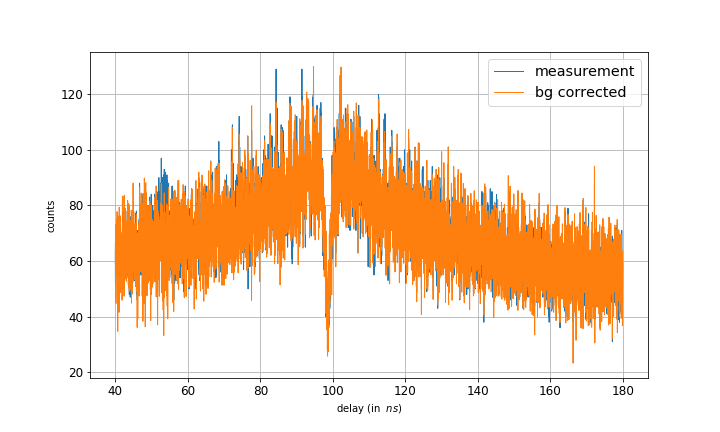
\includegraphics[width=\textwidth]{img/output_t2/2000.0muW_bg_vgl.png}
        \caption{}
        %label{fig_antibunch_raw_corr_comp}
    \end{subfigure}
    \caption{a: Antibunching measurement as recorded and compared to the adjusted background signal. b: Antibunching measurement as recorded and compared to the background corrected signal. The laser power is \SI{2000}{\micro W}.} %hoffe ok, dass der eine so doppelt ist
	%label{fig_antibunch_comp}
\end{figure}

\newpage
\subsection{Faraday Rotation additional figures}
\label{sec:anhang:far}

\begin{figure}[H]
    \centering
    \begin{subfigure}{0.47\textwidth}
        \centering
        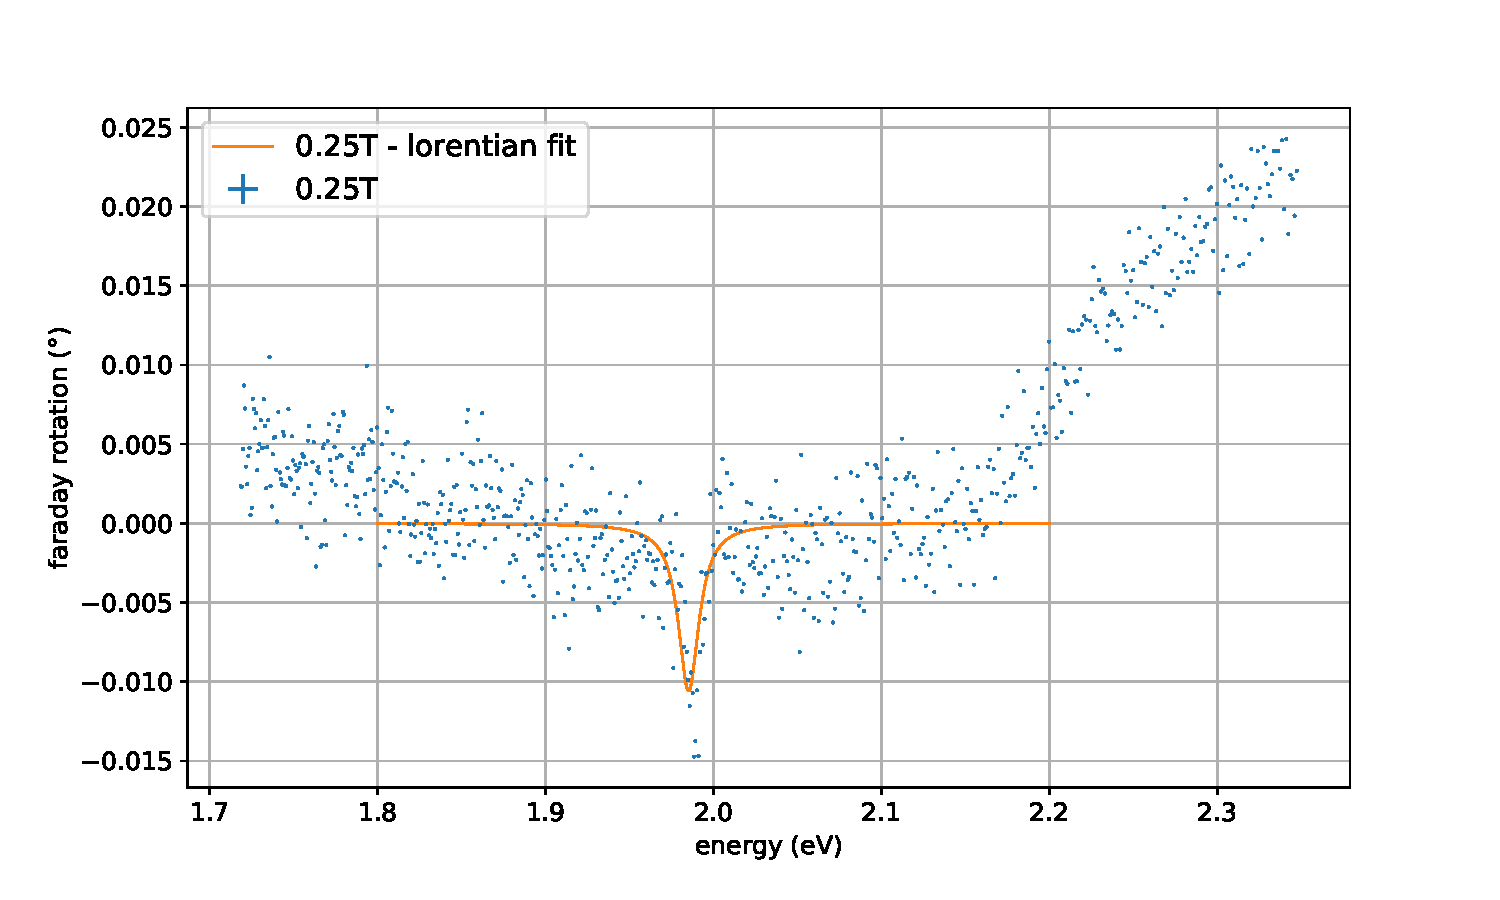
\includegraphics[width=1.0\textwidth]{plots/WS2_250mT.pdf}
    \caption{}
    %label{fig_antibunch_background_comp}
    \end{subfigure}
    %\hfill
    \begin{subfigure}{0.47\textwidth}
        \centering
        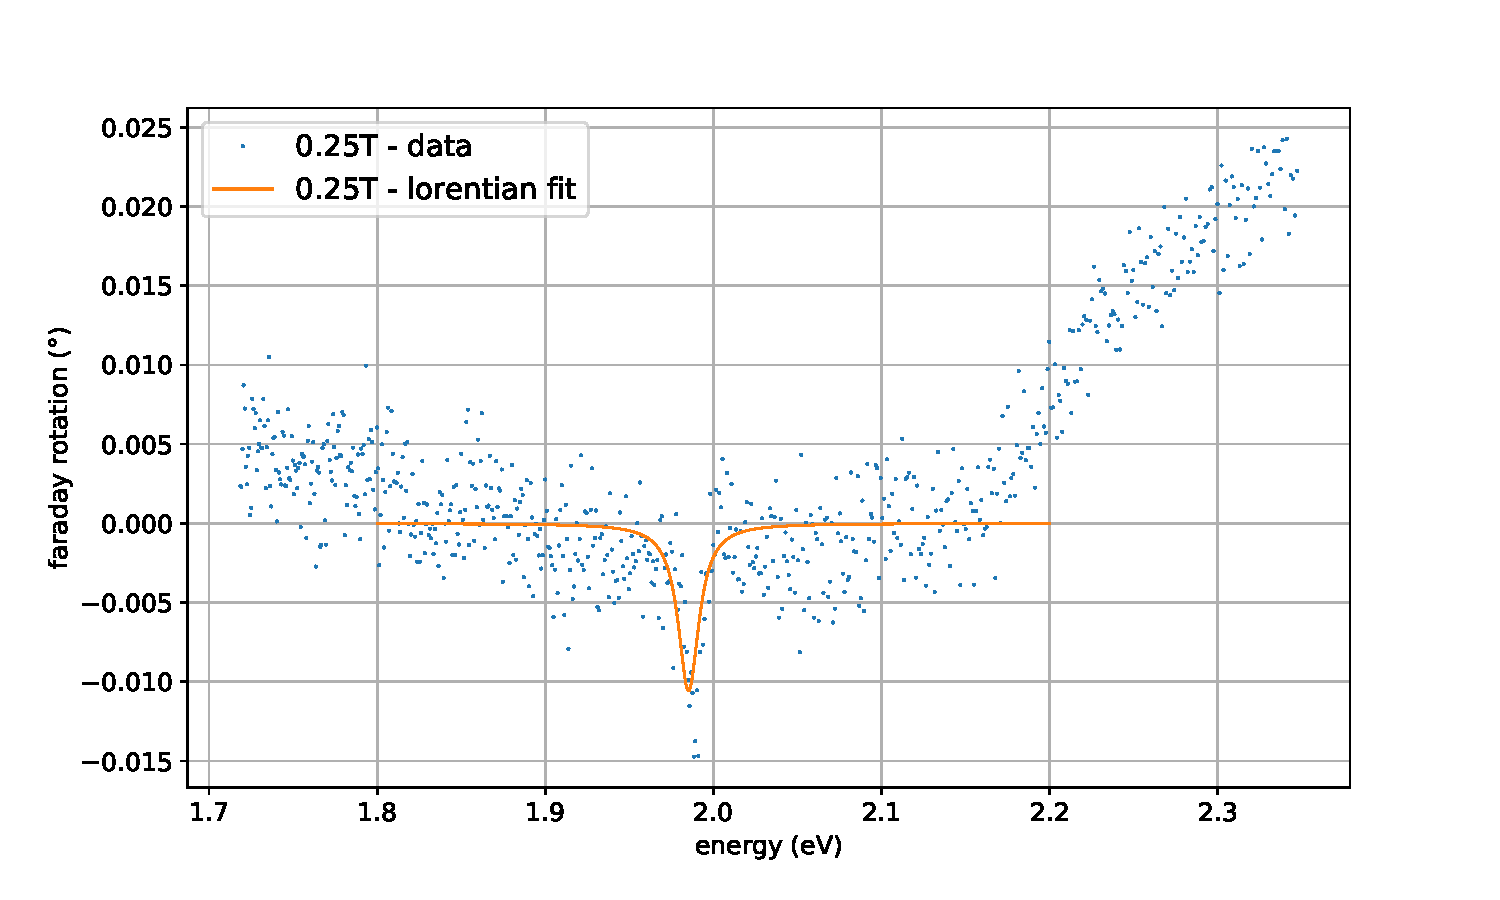
\includegraphics[width=\textwidth]{plots/WS2_250mT_noerror.pdf}
        \caption{}
        \label{fig_WS2_250mT_noerror}
    \end{subfigure}
    \caption{a: Representation of WS$_2$ monolayer data points of the faraday rotation with external magnetic field of \SI{0.25}{\tesla} and lorentian fit. b: Same as a, but without errorbars.} %hoffe ok, dass der eine so doppelt ist
\end{figure}

\begin{figure}[H]
    \centering
    \begin{subfigure}{0.47\textwidth}
        \centering
        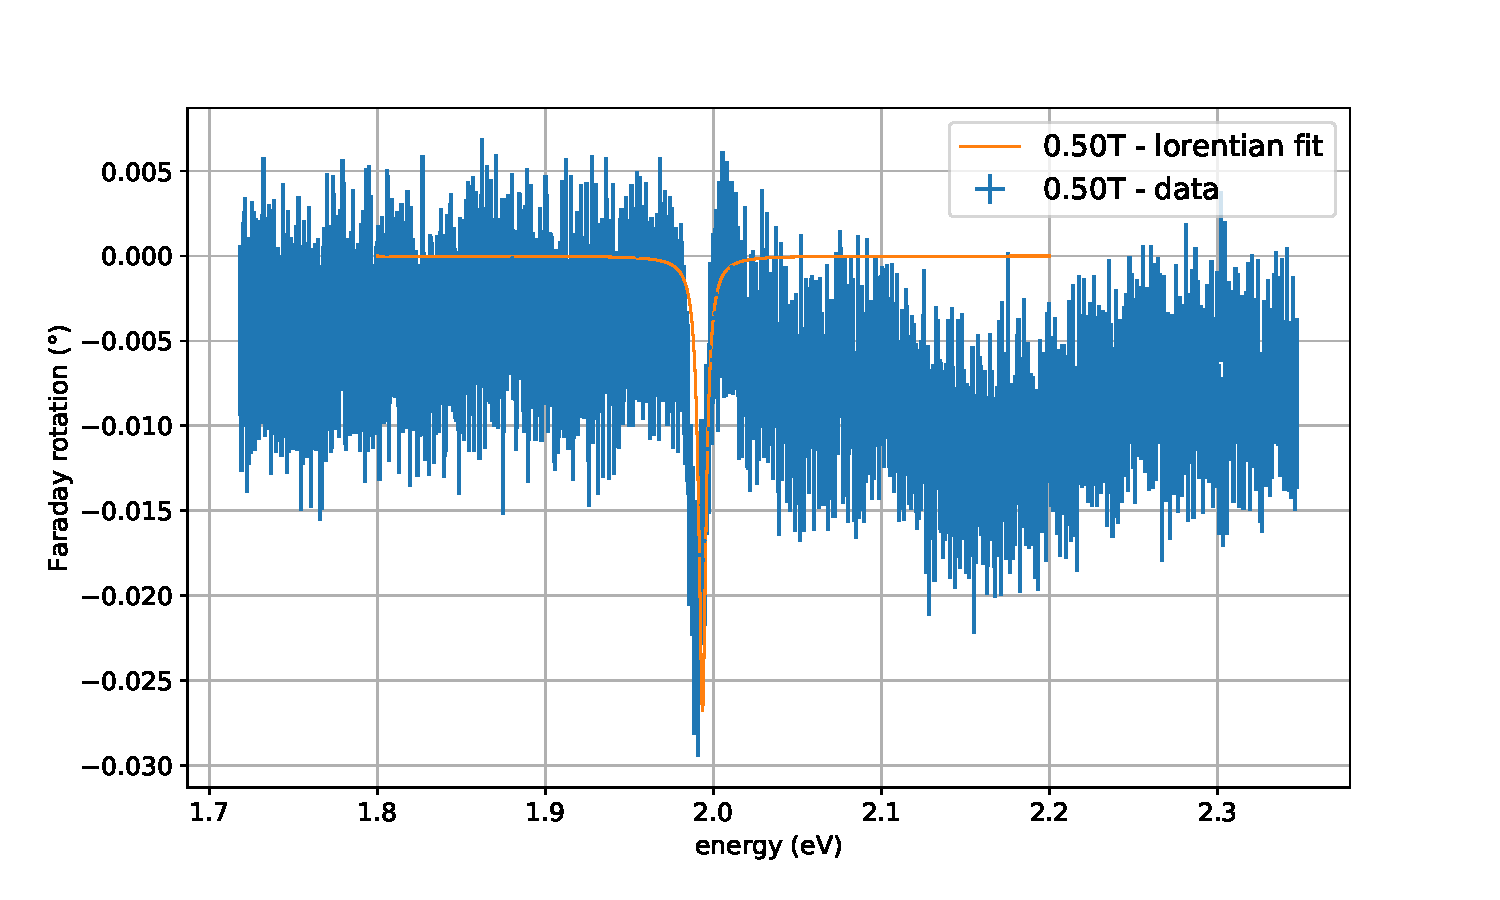
\includegraphics[width=1.0\textwidth]{plots/WS2_500mT.pdf}
    \caption{}
    %label{fig_antibunch_background_comp}
    \end{subfigure}
    %\hfill
    \begin{subfigure}{0.47\textwidth}
        \centering
        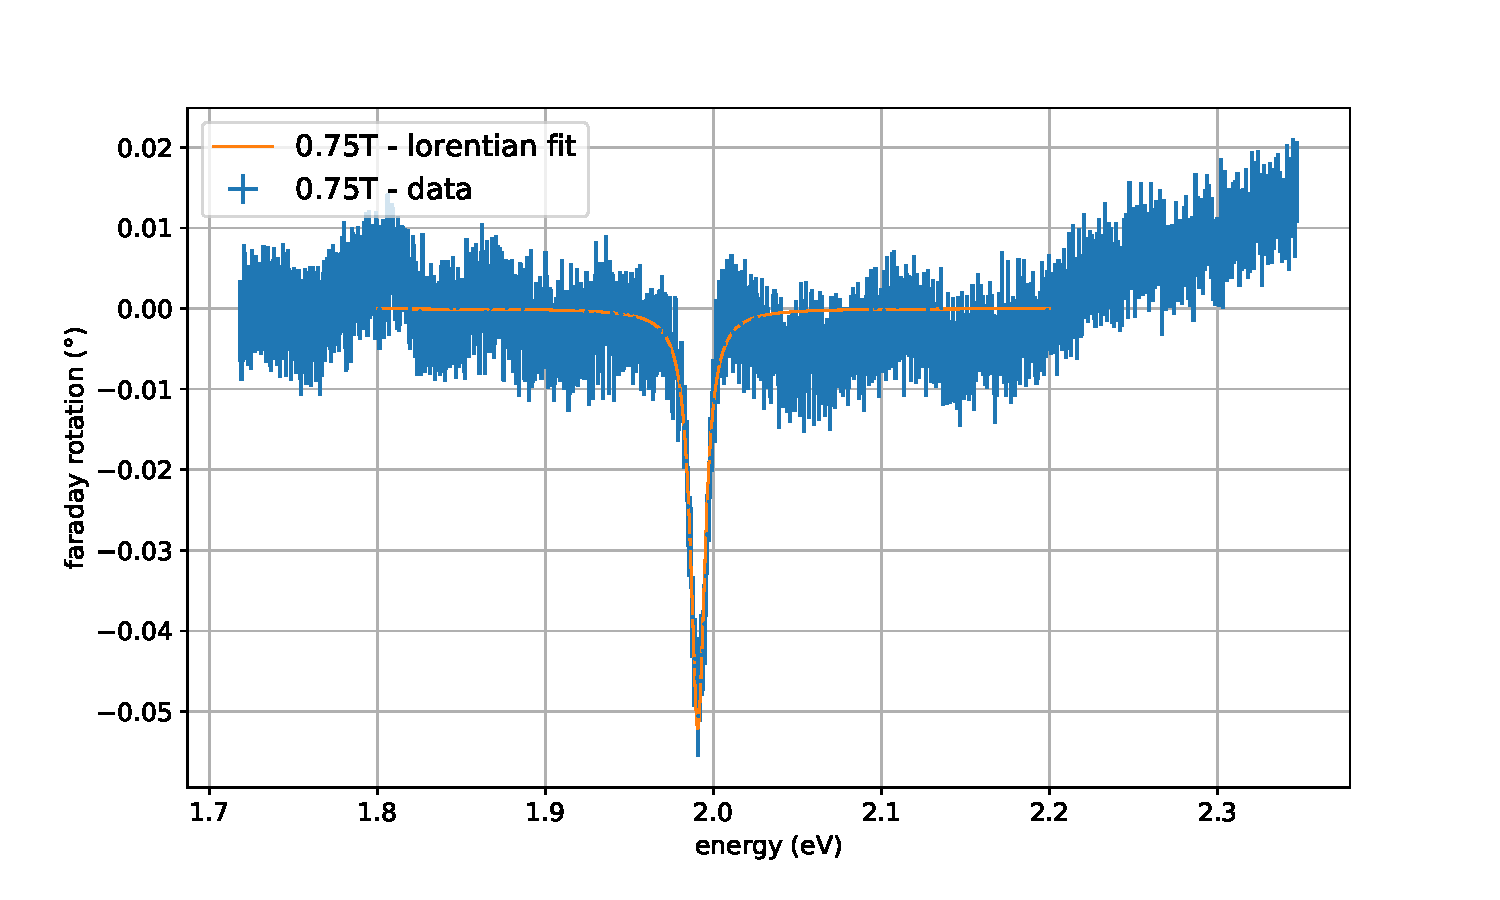
\includegraphics[width=\textwidth]{plots/WS2_750mT.pdf}
        \caption{}
    \end{subfigure}
    \caption{a: Representation of WS$_2$ monolayer data points of the faraday rotation with external magnetic field of \SI{0.50}{\tesla} and lorentian fit. b: Same as a, but at \SI{0.75}{\tesla}.} %hoffe ok, dass der eine so doppelt ist
\end{figure}

\begin{figure}[H]
    \centering
    \begin{subfigure}{0.47\textwidth}
        \centering
        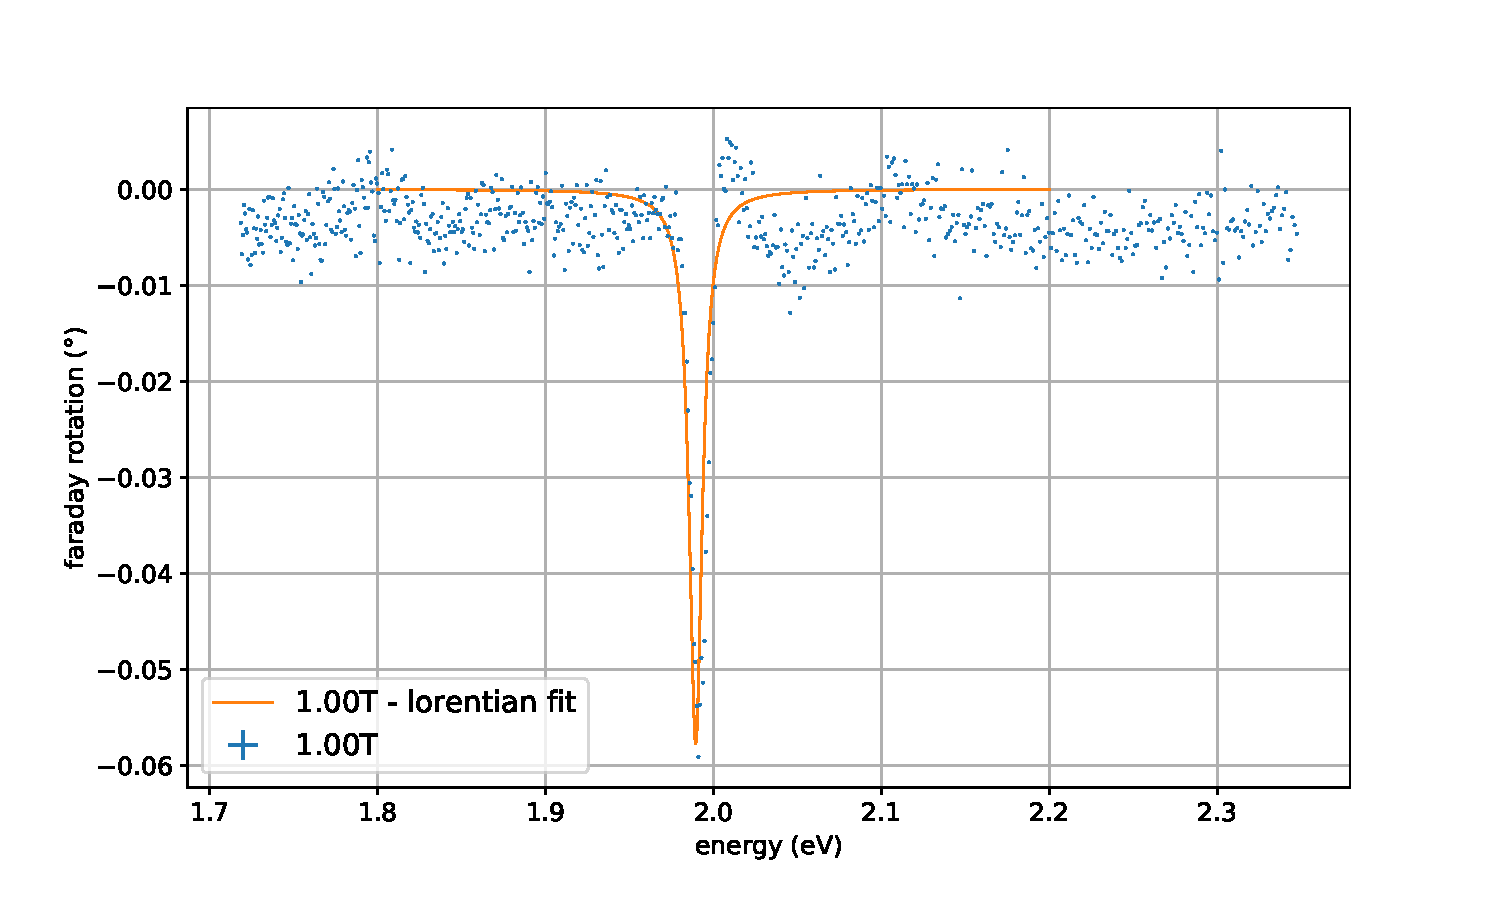
\includegraphics[width=1.0\textwidth]{plots/WS2_1000mT.pdf}
    \caption{}
    %label{fig_antibunch_background_comp}
    \end{subfigure}
    %\hfill
    \begin{subfigure}{0.47\textwidth}
        \centering
        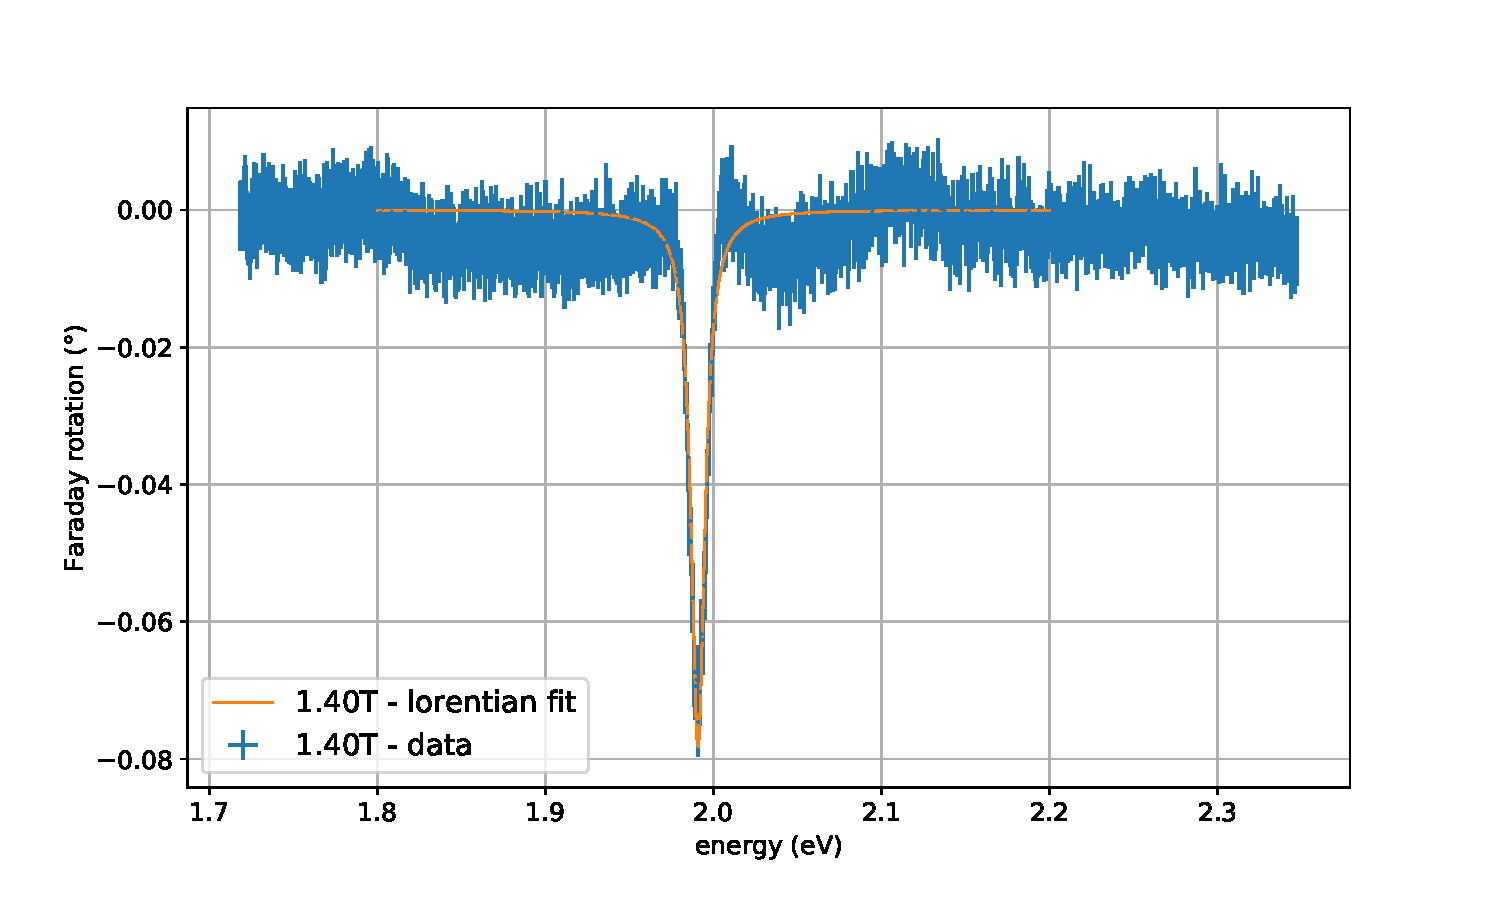
\includegraphics[width=\textwidth]{plots/WS2_1400mT.pdf}
        \caption{}
    \end{subfigure}
    \caption{a: Representation of WS$_2$ monolayer data points of the faraday rotation with external magnetic field of \SI{1.0}{\tesla} and lorentian fit. b: Same as a, but at \SI{1.4}{\tesla}.} %hoffe ok, dass der eine so doppelt ist
\end{figure}

	\printbibliography


\end{document}
